\documentclass[]{report}

% Pacotes para o português.
\usepackage[english]{babel}
\usepackage[utf8]{inputenc}
\usepackage[T1]{fontenc}

\usepackage{graphicx}     % Comando \includegraphics
\usepackage{xcolor}       % Comando de cores \textcolor
\usepackage{indentfirst}  % Indenta o primeiro parágrafo de cada seção
\usepackage{url}          % Comandos \url e \href
\usepackage[top=2cm, bottom=2cm, left=2cm, right=2cm]{geometry} % Define as margens do documento
\usepackage{multirow}     % Permite criar tabelas com uma célula ocupando várias linhas
\usepackage{amssymb}      % Símbolos matemáticos
\usepackage{amsmath}      % Ambientes para escrever fórmulas, \begin{align} por exemplo.
\usepackage{caption}      % Para definir o estilo das legendas de figuras e tabelas.
\usepackage{setspace}     % Para definir espaçamento entre linhas. (\onehalfspacing, \singlespacing, \doublespacing)
\usepackage{breakcites}   % Para permitir quebra de linha no meio de citações.
%\usepackage{times}        % Fonte Times New Roman
\usepackage{lipsum}       % Para gerar texto temporário. Exemplo: \lipsum \lipsum[1] \lipsum[4-5].
\usepackage{inconsolata}  % Fonte boa para códigos e URLs. Use \texttt{}
\usepackage{hyperref}     % Faz os links ficarem azuis e clicáveis. Facilita a navegação pelo PDF.
\usepackage{amsthm}
\usepackage{tikz, pgfplots}
\usepackage{subfigure}
\usepackage{float}

\makeatletter
\hypersetup{
	pdfkeywords={research project},
	colorlinks=true,       		% false: boxed links; true: colored links
	linkcolor=blue,          	% color of internal links
	citecolor=blue,        		% color of links to bibliography
	filecolor=magenta,      	% color of file links
	urlcolor=blue,
	bookmarksdepth=4,
}
\makeatother
	
\makeatletter
\renewcommand\tableofcontents{%         % Redefine table of contents to our taste
	\section*{\huge\centering\contentsname
		\@mkboth{%
			\MakeUppercase\contentsname}{\MakeUppercase\contentsname}}%
	\vspace{24pt}%
	\@starttoc{toc}%
	\newpage%
}

% Comando para marcar o texto para revisão.
\newcommand{\rev}[1]{\textcolor{red}{#1}}

% Permite escrever aspas normais "text" em vez de ``text''
\usepackage[autostyle]{csquotes}
\MakeOuterQuote{"}

	
\newcommand\underrel[2]{\mathrel{\mathop{#2}\limits_{#1}}}
	
\newcommand{\matriz}[1]{\hat#1}
	
\newcommand{\many}[2]{$#1_1, #1_2, \dots, #1_#2$}
	
\newcommand{\cmany}[3]{$#1_1 #3 #1_2 #3 \dots #3 #1_#2$}
	
\newcommand{\mmany}[2]{ #1_1, #1_2, \dots, #1_#2 }
	
\newcommand{\mcmany}[3]{#1_1 #3 #1_2 #3 \dots #3 #1_#2}
	
\newcommand{\set}[1]{\{#1\}}
	
\newcommand{\cjgt}[1]{\overline{#1}}
\DeclareMathOperator{\diag}{diag}
\DeclareMathOperator{\sign}{sign}
\DeclareMathOperator{\ai}{Ai}
\DeclareMathOperator{\re}{Re}
\DeclareMathOperator{\im}{Im}
\DeclareMathOperator{\Df}{D}
\DeclareMathOperator{\Ee}{E}
\DeclareMathOperator{\h}{h_1}
\DeclareMathOperator{\f}{f}
\DeclareMathOperator{\U}{U}
\DeclareMathOperator{\W}{W}
\DeclareMathOperator{\K}{K}
\DeclareMathOperator{\Hf}{\mathcal{H}}
\DeclareMathOperator{\Qf}{Q}
\DeclareMathOperator{\Gl}{\mathcal{L}}
\DeclareMathOperator{\g}{g}
\DeclareMathOperator{\V}{V}
\DeclareMathOperator{\Glin}{GL}
\newcommand{\iu}{\mathrm{i}\mkern1mu}
\renewcommand{\Im}{\mathop{\textrm Im}}
\DeclareMathOperator{\ee}{e}
\DeclareMathOperator{\supp}{supp}
\newcommand{\N}{\mathbb{N}}
\newcommand{\C}{\mathbb{C}}
\newcommand{\R}{\mathbb{R}}
\newcommand{\Z}{\mathbb{Z}}
\newcommand{\D}{\mathbb{D}}
\newcommand{\Q}{\mathbb{Q}}
\newcommand{\J}{J} %Jacobiano
\newcommand{\Id}{\mathbb{1}}
\newcommand{\p}{p} %medida
\newcommand{\E}{\mathbb{E}}
\newcommand{\Se}{\mathbb{S}}
\newcommand{\He}{\mathbb{H}}
\newcommand{\boh}{\mathit{o}}
\newcommand{\Boh}{\mathcal{O}}
\newcommand{\bbp}{\bm K_{\mathrm{BBP}}}
\newcommand{\ii}{\mathrm{i}}
\newcommand*{\deff}{\mathrel{\vcenter{\baselineskip0.5ex \lineskiplimit0pt
			\hbox{\scriptsize.}\hbox{\scriptsize.}}}%
	=}
\newcommand*{\revdeff}{=\mathrel{\vcenter{\baselineskip0.5ex \lineskiplimit0pt
			\hbox{\scriptsize.}\hbox{\scriptsize.}}}%
}
\newcommand{\dd}{\mathrm{d}}

% MATH DECLARATIONS
\newtheorem{lemma}{Lema}[section]
\newtheorem{thm}[lemma]{Theorem}
\newtheorem{claim}[lemma]{Afirmation}
\newtheorem{cor}[lemma]{Corolary}
\newtheorem{definition}[lemma]{Definition}
\newtheorem{conjecture}[lemma]{Conjecture}
\newtheorem{prop}[lemma]{Proposition}
\newtheorem{assumption}[lemma]{Assumption}
\numberwithin{equation}{section} %numeracao dentro de secoes
	
% PROOF ENV
\makeatletter
\newenvironment{Mproof}[1][Proof]{\par
	\pushQED{\qed}%
	\normalfont \topsep6\p@\@plus6\p@\relax
	\trivlist
	\item\relax
	{\itshape
		#1\@addpunct{.}}\hspace\labelsep\ignorespaces
}{%
	\popQED\endtrivlist\@endpefalse
}
\makeatother
%%%%%

% Title Page
\title{Notes on Master Studies}
\author{João Victor A. Pimenta}


\begin{document}
\maketitle

\begin{abstract}
	\textit{"En remontant chez moi pour y passer la soirée à travailler de mon mieux, je me disais que le monde n'est pas construit pour l'équilibre. Le monde est désordre. L'équilibre n'est pas la règle, c'est l'exception."\\
	G.Duhamel, Maitres, 1937}
\end{abstract}

\chapter{Asymptotic}

\section{Asymptotic on Integrals}

We will try to explore the asymptotic techniques on a specific type of function, as $\lambda \rightarrow \infty$, given by 

\begin{equation}
	\phi(\lambda) := \int_{\Gamma} g(s) \ee^{-\lambda f(s)} \dd s,
\end{equation}

where $\Gamma$ is a contour in the plane and $f, g$ are given \textcolor{red}{suitable} functions.

\subsection{Motivations}

\begin{itemize}
	\item Airy Equation $\psi''(x) = x \psi(x)$: Taking the Fourrier transform we have $$-\omega^2 \Phi(x) = \ii \Phi'(x)$$ for which we can solve for $\Phi(x) $ and then take the inverse Fourrier Transform to get $$\phi(x) = \frac{1}{2\pi} \int_{-\infty}^{\infty} \ee^{\ii/3 \omega^3 + \ii x \omega} \dd \omega.$$ The imaginary part of the argument is an odd function and therefore zero when integrated. The rest is expressed $$\phi(x) = \frac{1}{2\pi} \int_{-\infty}^{\infty} \cos{\left( \frac{\omega^3}{3} + x \omega \right)} \dd \omega.$$ But how to know if this is the only solution? One can prove that for a more general definition of a Transform $$\tilde{F} f(w) := \frac{1}{\sqrt{2\pi \ii}} \int_{\Gamma} \ee^{-\ii \omega s} f(s) \dd s$$ holds very similar properties of the Fourrier Tranformation and solves the equation for any contour that gives a convergent integral. We can actually choose independent contour such that each give us a different independent solution to the equation.
\end{itemize}

\section{Watson Lemma}

We start this study by looking at the functions $F: \R \rightarrow \R$
\begin{equation}
	F(\lambda) = \int_{0}^{T} f(t) \ee^{-\lambda t} \dd t
	\label{equation: F}
\end{equation}
which can be identified as the Laplace transform of a function $f$ supported on $[0,T]$.

\begin{thm}	
	(Watson's Lemma) Take $f \in L^1(0,T)$ and suppose that for some $\delta > 0$ it is of the form
	$$f(t) = t^\alpha f_0(t), \ \ 0 < t \leq \delta,$$
	where $\alpha \in (-1, \infty)$ and $f_0$ is continuously differentiable on $[0, \delta]$ with $f_0(0) \neq 0$. Then the function $F$ in \ref{equation: F} satisfies
	\begin{equation}
		F(\lambda) = \frac{f_0(0) \Gamma(\alpha + 1)}{\lambda^{\alpha + 1}} (1 + \Boh(\lambda^{-1}))
	\end{equation}
	when $\lambda \rightarrow \infty$ and where $\Gamma$ is the Gamma function.
\end{thm}

\begin{Mproof}
	A weak estimative of the integral values would be given by
	$$\int_{0}^{T} f(t) \ee^{-\lambda t} \dd t \leq ||f||_{L^1}$$
	where we only use the fact that $f \in L^1(0,T)$. However, we have more information on the behavior of the function in the section $0 < t < \delta$. To use this information we start by decomposing the function in two parts
	$$F(\lambda) = (1) + (2) = \int_{0}^{\delta} f(t) \ee^{-\lambda t} \dd t + \int_{\delta}^{T} f(t) \ee^{-\lambda t} \dd t.$$
	For $(2)$, we can use the weak estimative, leaving us with 
	$$F(\lambda) \leq \int_{0}^{\delta} f(t) \ee^{-\lambda t} \dd t + ||f||_{L^1} \ee^{-\delta \lambda}.$$
	Now, we remind of the condition of continous differentiability and the hypothesis on $f(t)$ to write $(1)$ as
	$$(1) = \int_{0}^{\delta} t^\alpha(f_0(0) + r(t)) \ee^{-\lambda t} \dd t = f_0(0) \int_{0}^{\delta} t^\alpha \ee^{-\lambda t} \dd t + \int_{0}^{\delta} t^\alpha r(t) \ee^{-\lambda t} \dd t = f_0(0) \cdot (1.1) + (1.2)$$
	For these two integrals we can try to simplify the problem by rewritring 
	$$(1.1) = \int_{0}^{\infty} t^\alpha \ee^{-\lambda t} \dd t - \int_{\delta}^{\infty} t^\alpha \ee^{-\lambda t} \dd t  = \frac{\Gamma(\alpha + 1)}{\lambda^{\alpha +1}} - \int_{\delta}^{\infty} t^\alpha \ee^{-\lambda t} \dd t $$
	$$|(1.2)| \leq ||f'||_{\infty} \int_{0}^{\delta} t^{\alpha + 1} \ee^{-\lambda t} \dd t = ||f'||_{\infty} \left( \int_{0}^{\infty} t^{\alpha+1} \ee^{-\lambda t} \dd t - \int_{\delta}^{\infty} t^{\alpha+1} \ee^{-\lambda t} \dd t \right) = ||f'||_{\infty} \left( \frac{\Gamma(\alpha + 2)}{\lambda^{\alpha +2}} - \int_{\delta}^{\infty} t^{\alpha+1} \ee^{-\lambda t} \dd t \right).$$
	We are now only missing one ingredient to get the result, the order of
	$$G(\lambda, \beta) \deff \int_{\delta}^{\infty} t^{\beta} \ee^{-\lambda t} \dd t, \ \ \ \lambda > 1, \ \ \ \beta > -1. $$
	Using Cauchy-Schwartz we can estimate
	\begin{equation*}
		\begin{split}
		|G(\lambda, \beta)|^2 & \leq \left( \int_{\delta}^{\infty} \ee^{-\lambda t} \dd t \right) \left(\int_{\delta}^{\infty} t^{2\beta} \ee^{-\lambda t} \dd t \right) \\
		& = \left(\frac{e^{-\lambda \delta}}{\lambda}\right) \left( \int_{\delta}^{\infty} t^{2\beta} \ee^{-\lambda t}\dd t \right)	\\
		& \stackrel{(u=\lambda t)}{=} \left(\frac{e^{-\lambda \delta}}{\lambda}\right) \left( \int_{\delta}^{\infty} \ee^{-u} u^{2\beta} \frac{1}{\lambda^{2\beta + 1}} \dd u \right) \\
		& = \frac{\ee^{-\lambda \delta}}{\lambda^{2\beta + 2}} M_\beta
		\end{split}
	\end{equation*}
	Where $M_\beta$ is independent of $\lambda$. That leave us with
	$$G(\lambda, \beta) = \Boh\left(\frac{\ee^{-\lambda\delta/2}}{\lambda^{\beta+1}}\right) = \Boh\left(\ee^{-\epsilon\lambda}\right)$$
	where $\epsilon > 0$ depends on $\beta$ and $\delta$. Finally we can rewrite
	$$(1.1) = \frac{\Gamma(\alpha + 1)}{\lambda^{\alpha +1}} - G(\lambda, \alpha) =  \frac{\Gamma(\alpha + 1)}{\lambda^{\alpha+1}} + \Boh\left(\ee^{-\epsilon\lambda}\right)$$
	$$|(1.2)| \leq ||f'||_{\infty} \left( \frac{\Gamma(\alpha + 2)}{\lambda^{\alpha +2}} - G(\lambda, \alpha + 1) \right) = ||f'||_{\infty} \left( \frac{\Gamma(\alpha + 2)}{\lambda^{\alpha +2}} + \Boh\left(\ee^{-\epsilon\lambda}\right) \right) = \Boh\left(\lambda^{-\alpha-2}\right)$$
	and finally
	$$F(\lambda) \leq \Boh\left(\lambda^{-\alpha-2}\right) + f_0(0) \left( \frac{\Gamma(\alpha + 1)}{\lambda^{\alpha+1}} + \Boh\left(\ee^{-\epsilon\lambda}\right) \right) + ||f||_{L^1} \ee^{-\delta \lambda}.$$
	by the dominance of the exponential error, we can finally get the result
	$$F(\lambda) = \frac{f_0(0) \Gamma(\alpha + 1)}{\lambda^{\alpha + 1}} (1 + \Boh(\lambda^{-1}))$$
\end{Mproof}

In the estimative the Gamma function and the factor of $\lambda^-1$ is the result of integrating the linear exponent of $\ee$ given by $-\lambda t$. If we, however, change this exponent to be of the general type $-\lambda t^d$ we can still have a similar result on the behavior of the function.

\begin{prop}	
	For $T, S > 0$, define the function
	$$G(\lambda) \deff \int_{-S}^{T} g(t) \ee^{-\lambda t^2} \dd t$$
	and assume $g(x)$ absolutely integrable in $[-S, T]$, of class $C^1$ in a fixed neighborhood of the origin. Then the function satisfies
	\begin{equation}
		G(\lambda) = \frac{g(0) \Gamma(1/2)}{\lambda^{1/2}} + \Boh \left(\frac{1}{\lambda^{3/2}} \right)
	\end{equation}
	when $\lambda \rightarrow \infty$ and where $\Gamma$ is the Gamma function.
	\label{prop: cor watson}
\end{prop}

\begin{Mproof}
	The proof is a reduction of the problem to Watson's Lemma. Assume, $T>S$ and write
	$$G(\lambda) = \int_{-S}^{S} g(t) \ee^{-\lambda t^2} \dd t + \int_{S}^{T} g(t) \ee^{-\lambda t^2} \dd t $$
	The second integral we know to be of order
	$$\int_{S}^{T} g(t) \ee^{-\lambda t^2} \dd t \leq ||g||_{\infty} \ee^{-\lambda S^2},$$
	exponential on $\lambda$, so we drop it. For the first integral we rewrite
	\begin{equation*}
		\begin{split}
			\int_{-S}^{S} g(t) \ee^{-\lambda t^2} \dd t & = \int_{0}^{S} (g(t) + g(-t)) \ee^{-\lambda t^2}\dd t \\
			& \stackrel{(u= t^2)}{=} \frac{1}{2} \int_{0}^{S^2} \left(\frac{g\left(\sqrt{u}\right) + g\left(-\sqrt{u}\right)}{\sqrt{u}}\right) \ee^{-\lambda u} \dd u
		\end{split}
	\end{equation*}
	where now we can use Watson's Lemma.
\end{Mproof}

\section{Laplace's Method}

A seemly natural extension of the type of function we were dealing with are functions of the type
\begin{equation}
	\Phi(\lambda) \deff \int_{a}^{b} g(t) \ee^{-\lambda \phi(t)} \dd t
	\label{equation: Laplace}
\end{equation}
for $a,b \in \R \cup \{-\infty, \infty\}$ and $a<b$. For now, $\phi$ is a real-valued function. To begin the study let's make some assumptions. The first one is that $a$ is finite, that means that we can set $a=0$ without loss of generality. The second assumption is that $\phi$ is a increasing function on $[0,b]$, so that $\phi(0) < \phi(t)$ for any $t$ in the interval. With that we note that the coefficient $\ee^{-\lambda \phi(t)} / \ee^{-\lambda \phi(0)}$ decreases exponentially, that is, the integral is accumulated as the neighborhood of $0$,
$$\Phi(\lambda) \approx \int_{0}^{\delta} g(t) \ee^{-\lambda \phi(t)} \dd t.$$
As we know $\phi(t)$ to be increasing, it's first non zero derivative must be of even order, so that when we expanded the function by Taylor, 
$$\phi(t) \approx \phi(0) + \phi_{2k+1} t^{2k+1}$$
for some $k\geq 0$ and $|t| < \delta$. As $\phi_{2k+1}$, the $(2k+1)$th-derivative, must be positive we also have that, as $\lambda \rightarrow \infty$,
\begin{equation*}
	\begin{split}
		\Phi(\lambda) & \approx \ee^{-\lambda \phi(0)} \int_{0}^{\delta} g(t) \ee^{-\lambda \phi_{2k+1}(t) \cdot t^{2k+1}} \dd t\\
		& \stackrel{(u=t(\lambda \phi_{2k+1})^{1/(2k+1)})}{\approx} \ee^{-\lambda \phi(0)} \frac{g(0)}{(\lambda \phi_{2k+1})^{\frac{1}{2k+1}}} \int_{0}^{\infty} \ee^{-u^{2k+1}} \dd u \\
		& \stackrel{(s=u^{2k+1})}{\approx} \ee^{-\lambda \phi(0)} \frac{g(0)}{ (2k+1)(\lambda \phi_{2k+1})^{\frac{1}{2k+1}}} \int_{0}^{\infty} \ee^{-s} \dd u
	\end{split}
\end{equation*}
Where the integral can be evaluated as an Gamma function.

More than anything we need to focus on an important assumption that was made: that $\phi$ has a global minima at one of the endpoints of integration. Is that were not the case, for example if $a < 0 < b$ and $\phi(t)$ had a global minima at $t=0$ we would now have to consider the expansion
$$\phi(t) \approx \phi(0) + \phi_{2k} t^{2k}$$
which would lead us to the expression
$$\Phi(\lambda) \approx \ee^{-\lambda \phi(0)} \frac{g(0)}{(\lambda \phi_{2k})^{\frac{1}{2k}}} \int_{-\infty}^{\infty} \ee^{-u^{2k}} \dd u$$
which differentiates of the previously result more importantly by the limits of integration. This is closely related to physical boundaries of the problem.

\begin{thm}
	(Laplace's Method, endpoint contributions) Let $\Phi$ be as in \ref{equation: Laplace}, with a finite and $g \in L^1(a,b)$. Assume that $\phi$ has a unique global minimum at $t=a$. In addition, suppose that for some $\delta > 0$ and some $\alpha > -1$, the function $g$ takes the form
	$$ g(t) = (t-a)^{\alpha} g_0(t)$$
	for $|t-a| < \delta$ and $g_0$ continuously differentiable in $[a, a+\delta]$ and $g_0(a) \neq 0$, whereas $\phi$ is twice continuously differentiable on $[a, a+\delta]$ with $\phi'(a) > 0$. Then the function $\Phi$ satisfies an estimate of the form
	\begin{equation}
		\Phi(\lambda) = \frac{1}{\lambda^{\alpha + 1}} \frac{g_0(a) \Gamma(\alpha + 1)}{\phi'(a)^{\alpha + 1}} \ee^{-\lambda \phi(a)} \left(1+\Boh(\lambda^{-1})\right)
	\end{equation}
	as $\lambda \rightarrow \infty$.
\end{thm}

\begin{Mproof}
	Start by assuming, w.l.g, that $a=0$ and dividing the integral in two, one in the region of interest and one in the rest of the interval
	$$\Phi(\lambda) = \int_{0}^{b} g(t) \ee^{-\lambda \phi(t)} \dd t = \int_{0}^{\delta} g(t) \ee^{-\lambda \phi(t)} \dd t + \int_{\delta}^{b} g(t) \ee^{-\lambda \phi(t)} \dd t = (1) + (2).$$
	Knowing that $\phi$ has a global minima at $t = 0$ we can assume, changing $\delta$ as needed, that $\phi(t) > \phi(\delta)$ for any $t > \delta$. That give us a simple limitation for $(2)$:
	$$(2) = \int_{\delta}^{b} g(t) \ee^{-\lambda \phi(t)} \dd t \leq \ee^{-\lambda \phi(\delta)} \int_{\delta}^{b} g(t) \dd t \leq \ee^{-\lambda \phi(\delta)} ||g||_{L^1[0,b]}.$$
	We now get back to $(1)$ and start by studying the difference give by $\phi(t) - \phi(0) = s$ in a similar way that we would think of a change of variable. Define the multivariate function 
	$$H(t,s) \deff \phi(t) - \phi(0) - s$$
	such that $H(0,0) = 0$ and $\partial_t H(0,0) \neq 0$ so that we can use the Theorem of Implicit Function to say that there exists a unique bijective and continuously differentiable function $t(s) \deff t$ such that 
	\begin{equation*}
		\begin{cases}
		\phi(t(s)) - \phi(0) - s = 0	\\
		t'(0) = \frac{\partial_s H(0,0)}{\partial_t H(0,0)} = \frac{1}{\phi'(0)} 
		\end{cases}
	\end{equation*}
	If we set $T = t^{-1}(\delta)$ we would then have
	$$\int_{0}^{\delta} g(s) \ee^{-\lambda \phi(s)} \dd s = \int_{0}^{T} g(t(s)) \ee^{-\lambda \phi(t(s))} t'(s) \dd s$$
	for now to apply the assumption on $g$. We write $g(t(s)) = t^\alpha(s) g_0(t(s))$ and because of Taylor,
	$$t(s) = s t'(0) (1+r(s)) = \frac{s}{\phi'(0)}(1+r(s)).$$
	Joining both results,
	\begin{equation}
		\begin{split}
			\int_{0}^{T} g(t(s)) \ee^{-\lambda \phi(t(s))} t'(s) \dd s & = \ee^{\lambda \phi(0)} \int_{0}^{T} g(t(s)) \ee^{-\lambda (\phi(t(s)) - \phi(0))} t'(s) \dd s \\
			& = \ee^{\lambda \phi(0)} \int_{0}^{T} t^\alpha(s) g_0(t(s)) \ee^{-\lambda s} t'(s) \dd s \\
			& = \frac{\ee^{\lambda \phi(0)}}{\phi'(0)^\alpha} \int_{0}^{T} s^\alpha (1+r(s))^\alpha g_0(t(s)) \ee^{-\lambda s} t'(s) \dd s			
		\end{split}
	\end{equation}
	where, if we set $f(s) \deff s^\alpha (1+r(s))^\alpha g_0(t(s))$ we can apply Watson's Lemma.
\end{Mproof}

\begin{thm}
	(Laplace's Method, interior contributions) Let $\Phi$ be as in \ref{equation: Laplace}, with a finite and $g \in L^1(a,b)$. Assume that $\phi$ has a unique global minimum at $t=c \in (a,b)$. In addition, suppose that for some $\delta > 0$ and some $\alpha > -1$, the function $g$ takes the form
	$$ g(t) = (t-a)^{\alpha} g_0(t)$$
	for $|t-a| < \delta$ and $g_0$ continuously differentiable in $[c-\delta, c+\delta]$ and $g_0(a) \neq 0$, whereas $\phi$ is three times continuously differentiable on $[c-\delta, c+\delta]$ with $\phi'(a) > 0$. Then the function $\Phi$ satisfies an estimate of the form
	\begin{equation}
		\Phi(\lambda) = \ee^{-\lambda \phi(c)} \left( \frac{\sqrt{2\pi} g(c)}{\sqrt{|\phi''(c)|}\lambda^{1/2}} + \Boh(\lambda^{-3/2})\right)
	\end{equation}
	as $\lambda \rightarrow \infty$.
	\label{prop: (Laplace's Method, interior contributions)}
\end{thm}

\begin{Mproof}
	Although the proof may be similar there is an important distinction in the solution. Suppose we wanted to try the same approach. We would first assume, w.l.g., that c = 0. Then, we could write
	$$ \Phi(\lambda) = \int_{a}^{b} g(t) \ee^{-\lambda \phi(t)} \dd t = \int_{a}^{-\delta} g(t) \ee^{-\lambda \phi(t)} \dd t + \int_{-\delta}^{\delta} g(t) \ee^{-\lambda \phi(t)} \dd t + \int_{\delta}^{b} g(t) \ee^{-\lambda \phi(t)} \dd t = (1) + (2) + (3).$$
	For $(1)$ and $(3)$ the result is as it was before
	\begin{equation*}
	\begin{cases}
		(1)	= \int_{\delta}^{a} g(-t) \ee^{-\lambda \phi(-t)} \dd t \leq \ee^{\lambda \phi(-\delta)} ||g||_{L^1[a,b]}\\
		(3) = \int_{\delta}^{b} g(t) \ee^{-\lambda \phi(t)} \dd t \leq \ee^{\lambda \phi(\delta)} ||g||_{L^1[a,b]}
	\end{cases}
	\end{equation*}
	For $(2)$ we would try to define a function 
	$$H(t,s) \deff \phi(t) - \phi(0) - s^2.$$
	However we could not apply the Implicit Function Theorem here as its derivative $\partial_t H = \phi'$ vanishes at $t=0$. A nice fact about this indetermination is that it doesn't come from the fact that there are no solutions to $H(t,s) = 0$ but from the fact that there are two. To solve this we will use a technique called \textit{blow up}. First, we introduce a variable $v = v(t)$ such that $vs = t$. Now, we redefine our function of interested to be
	$$L(s, v) \deff \frac{\phi(sv) - \phi(0)}{s^2} - 1.$$
	for $s\in(-\delta, \delta) - \{0\}$. We would think this function is also singular but note that, using the Taylor Expansion of $\phi$ we can write
	$$\phi(t) = \frac{\phi''(0)}{2}t^2 + t^3R(t) $$
	which leave us with 
	$$L(s, v) = \frac{\phi''(0)}{2}v^2 + sv^3R(sv) - 1 $$
	where we can indeed apply the Implicit Function Theorem. In fact, we know $L \in C^2$ and as we want to solve for $L(s,v) = 0$, we need that the $v_0$ we take to satisfy $L(0, v_0) = 0$, ie,
	$$v_0 = \sqrt{\frac{2}{\phi''(0)}}.$$
	Now, we also know that
	$$\partial_v L(0, v_0) = \phi''(0) v_0 \neq 0.$$
	So we get a bijective and continuously differentiable function $v = v(s)$ such that
	\begin{equation*}
	\begin{cases}
		L(s, v(s)) = 0 \\
		v(0) = v_0
	\end{cases}
	\end{equation*}
	But, $L(s, v(s))$ means exactly that
	$$\phi(t) - \phi(0) = s^2$$
	with $t = t(s) = sv(s)$. Getting back to our equation, we have that
	$$ \ee^{\lambda \phi(0)} \int_{-\delta}^{\delta} g(t) \ee^{-\lambda (\phi(t)-\phi(0))} \dd t = \ee^{\lambda \phi(0)} \int_{\alpha}^{\beta} g(sv(s)) (v(s) + sv'(s)) \ee^{-\lambda s^2} \dd t$$
	where we can easily calculate $\alpha = - \sqrt{\phi(-\delta) - \phi(0)}$ and $\beta = \sqrt{\phi(\delta) - \phi(0)}$. We finish the prove with Proposition \ref{prop: cor watson}.
\end{Mproof}

\subsection{Example - Gamma Function}

Take the function called Gamma given by the expression

\begin{equation}
	\Gamma(x) = \int_{0}^{\infty} \ee^{-t} t^{x-1} \dd t
	\label{eq: Gamma}
\end{equation}

We are interested in what happens to the function when we take the variable $x$ to $+\infty$. To see what happens, let's fit it into Proposition \ref{prop: (Laplace's Method, interior contributions)}. Rewrite equation \ref{eq: Gamma} as
$$\int_{0}^{\infty} \ee^{-t+x\log{(t)}-\log{(t)}} \dd t.$$ 
This lead us to identify $\phi$ as $-\log{(t)}$, which would give us $\phi'(t) < 0$, that is, we would have it's minimum at $t=+\infty$. However $\ee^{\log{(t)}} = t^1$ is not integrable near the origin. Something need to change about the identification. Let's introduce a variable to rescale the integral: $xs = t$, s.t.,
$$\Gamma(x) = x^x \int_{0}^{\infty} \ee^{-\lambda(s - \log{(s)})} \ee^{-s} \dd s.$$
Where we have used $\lambda = x - 1$. Thus we identify $\phi(s) = s - \log(s)$ and $g(s) = \ee^{-s}$. in fact, now $\phi$ has a global minima at $s = 1$ and $\phi''(1) = 1 \neq 0$. Hence
\begin{equation*}
	\begin{split}
		\Gamma(x) & = \frac{\sqrt{2\pi} x^x \ee^{-x}}{(x-1)^{(-1/2)}} (1 + \Boh(x^{-1})) \\
		& = \sqrt{2\pi} x^{x - 1/2} \ee^{-x} (1 + \Boh(x^{-1})) \\
		& = (x-1/2)\log{(x)} - x + \frac{1}{2} \log{(2\pi)}
	\end{split}
\end{equation*} 
Which is called the Stirling formula.

\section{Steepest Descent}

Let's now finally explore integrals over the complex plane with complex valued functions. We retake the integral 
\begin{equation}
	\phi(\lambda) := \int_{\Gamma} g(s) \ee^{-\lambda f(s)} \dd s,
	\label{eq: general int}
\end{equation}
where $\Gamma$ is a contour in the complex plane and $f, g$ are given \textit{complex-valued, analytic functions.}

Suppose that $\Gamma$ is parametrized by $\gamma : [a,b] \rightarrow \C$ and let us decompose the functions we have into their real and imaginary parts such as
$$f(z) = u(z) + \ii v(z), \ \ g(z) = p(z) + \ii q(z), \ \ \gamma(t) = \alpha(t) + \ii \beta(t)$$
with all functions in the decomposition being real valued. Of course we now have 
$$\ee^{-\lambda f(z)} = \ee^{-\lambda u(z)} \ee^{-\ii v(z)}$$
and when $\lambda$ grows large, we have the exponentially growing/decaying term $\ee^{-\lambda u(z)}$ and a oscillating term coming from $\ee^{\ii v(z)}$ which is hard to control. The idea to get around this fact is to use paths in which this term is constant. If we have such a case, we would write

\begin{equation}
	\Phi(\lambda) = \ee^{-\ii \lambda v_0} \int_{a}^{b} (p(\gamma(t))\alpha'(t)-q(\gamma(t))\beta'(t)) \ee^{-\lambda u(\gamma(t))} \dd t + \ii \ee^{-\ii \lambda v_0} \int_{a}^{b} (p(\gamma(t))\beta'(t)-q(\gamma(t))\alpha'(t)) \ee^{-\lambda u(\gamma(t))} \dd t
	\label{eq: decomposition}
\end{equation}
where each integral can now be solved by Laplace's method.

\begin{thm}
	Consider $\Phi$ as in \ref{eq: general int} with a smooth contour $\Gamma$. Assume that the exponent $f = u + \ii v$ is an analytic function on a neighborhood of $\Gamma$ that satisfies
	$$v(z) \equiv v_0, \ \ \ z \in \Gamma$$
	In addition, suppose that $u$ has a unique minimum at an interior point of $\Gamma$, say on $z_0 \in \Gamma$, with $f''(z_0) \neq 0$, and also that $g$ is analytic on a neighborhood of $\Gamma$  and satisfies
	$$\int_{\Gamma} |g(z)| |dz| < \infty.$$
	Then $\Phi$ has a leading asymptotic as $\lambda \rightarrow +\infty$ given by
	$$\Phi(\lambda) = \ee^{-\lambda f(z_0)} \left(\frac{\sqrt{2\pi}g(z_0)\ee^{\ii \theta(z_0)}}{\lambda^{1/2}\sqrt{|f''(z_0)|}} + \Boh(\lambda^{-3/2}) \right), \ \ \lambda \rightarrow + \infty,$$
	where $\theta(z_0)$ is the angle of the oriented tangent of $\Gamma$ at $z_0$.
\end{thm}

\begin{Mproof}
		Fix a parametrization $\gamma : [a,b] \rightarrow \C$ of $\Gamma$ with $\gamma(c) = z_0, a < c < b$, and decompose $\Phi$ as before in $\ref{eq: decomposition}$. By the assumptions on the functions $f, g$ we can apply Laplace`s method on both equations, and yields, as $\lambda \rightarrow + \infty$,
		$$\int_{a}^{b} (p(\gamma(t))\alpha'(t)-q(\gamma(t))\beta'(t)) \ee^{-\lambda u(\gamma(t))} \dd t = \sqrt{2\pi} \ee^{-\lambda u(z_0)} \left( \frac{p(z_0)\alpha'(c)-q(z_0)\beta'(c)}{\sqrt{|(u \circ \gamma)''(c)|} \lambda^{1/2}} + \Boh \left(\lambda^{3/2}\right) \right)$$
		and
		$$\int_{a}^{b} (p(\gamma(t))\beta'(t)-q(\gamma(t))\alpha'(t)) \ee^{-\lambda u(\gamma(t))} \dd t = \sqrt{2\pi} \ee^{-\lambda u(z_0)} \left( \frac{p(z_0)\beta'(c)-q(z_0)\alpha'(c)}{\sqrt{|(u \circ \gamma)''(c)|} \lambda^{1/2}} + \Boh \left(\lambda^{3/2}\right) \right)$$
		Using that $v_0 + u(z_0) = f(z_0)$ and also that,
		$$ (p(z_0)\alpha'(c)-q(z_0)\beta'(c)) + \ii (p(z_0)\beta'(c)-q(z_0)\alpha'(c)) = g(z_0)\gamma'(c).$$
		Combining the estimative for both parts we get
		$$\Phi(\lambda) = \sqrt{2\pi} \ee^{-\lambda f(z_0)} \left( \frac{g(z_0)\gamma'(c)}{\sqrt{|(u \circ \gamma)''(c)|} \lambda^{1/2}} + \Boh \left(\lambda^{3/2}\right) \right)$$ 
		and it suffices now to get an expression for the second derivative in the denominator. Knowing the imaginary part is constant we can write
		$$\frac{\dd}{\dd t} u(\gamma(t)) = \frac{\dd}{\dd t} f(\gamma(t)) = \gamma'(t) f'(\gamma(t))$$
		and
		$$ \frac{\dd^2}{\dd t} u(\gamma(t)) = \frac{\dd^2}{\dd t} f(\gamma(t)) = (\gamma'(t))^2 f''(\gamma(t)) + \gamma''(t) f'(\gamma(t)).$$
		Hence,
		$$ \frac{\gamma'(c)}{\sqrt{|(u \circ \gamma)''(c)|}} = \frac{1}{\sqrt{|f''(z_0)|}} \frac{\gamma'(c)}{|\gamma'(c)|}$$
		which concludes the proof.
\end{Mproof}

We now need do discuss why this assumption of constant value of $\Im(f(z))$ is not an assumption as strong as one might assume at first. Suppose we want to integrate in a random contour $\Gamma$ of the plane. Of course, our assumption that the functions were analytic permit us to deform the contour keeping the value of the integral. We are going to use this to find an contour $\tilde{\Gamma}$ such that sections of the contour are such that $\Im(f(z))$ is constant. in the figure above we plot such a scenario by using the level lines of the imaginary part of $f$ as curves on the plane. 

\begin{figure}[h]
	\centering
	\subfigure{
	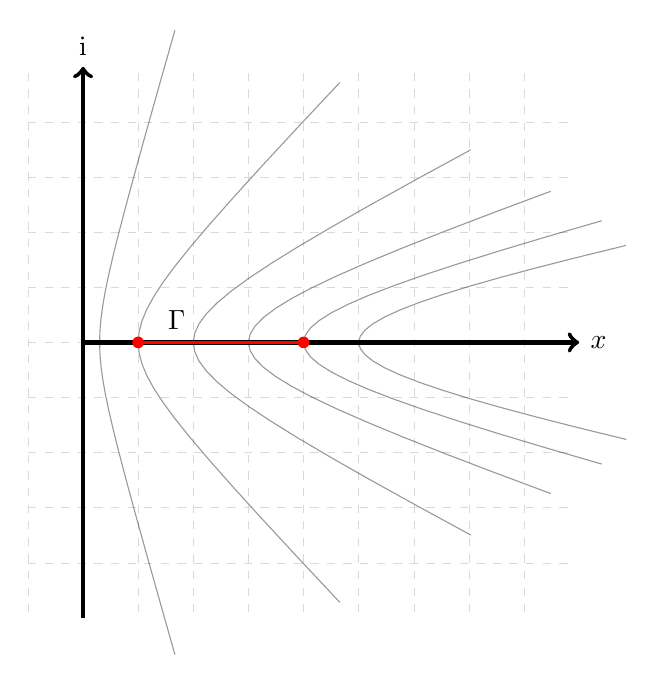
\begin{tikzpicture}[scale=.7]
	\draw[help lines, color=gray!30, dashed] (-1,-4.9) grid (8.9,4.9);
	\draw[->,ultra thick] (0,0)--(9,0) node[right]{$x$};
	\draw[->,ultra thick] (0,-5)--(0,5) node[above]{$\ii$};
	\pgfmathsetmacro{\e}{1.44022}   % eccentricity
	\pgfmathsetmacro{\a}{1}
	\pgfmathsetmacro{\b}{(\a*sqrt((\e)^2-1)} 
	\draw[opacity=0.4] plot[domain=-2.4:2.4] ({0.3*\a*cosh(\x)},{\b*sinh(\x)});
	\draw[opacity=0.4] plot[domain=-2.22:2.22] ({1*\a*cosh(\x)},{\b*sinh(\x)});
	\draw[opacity=0.4] plot[domain=-1.93:1.93] ({2*\a*cosh(\x)},{\b*sinh(\x)});
	\draw[opacity=0.4] plot[domain=-1.7:1.7] ({3*\a*cosh(\x)},{\b*sinh(\x)});
	\draw[opacity=0.4] plot[domain=-1.5:1.5] ({4*\a*cosh(\x)},{\b*sinh(\x)});
	\draw[opacity=0.4] plot[domain=-1.3:1.3] ({5*\a*cosh(\x)},{\b*sinh(\x)});
	\node (Gamma) at (1.7,0.4)    {$\Gamma$};
	\draw[color=red, very thick] (1,0) -- (4,0);
	\fill[color=red] (1,0) circle (3pt);
	\fill[color=red] (4,0) circle (3pt);
	\end{tikzpicture}
	}
	\subfigure{
	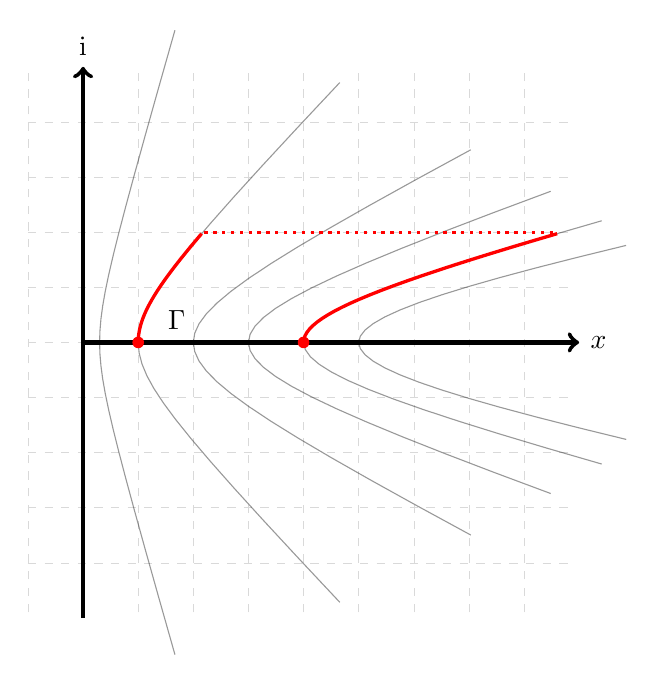
\begin{tikzpicture}[scale=.7]
		\draw[help lines, color=gray!30, dashed] (-1,-4.9) grid (8.9,4.9);
		\draw[->,ultra thick] (0,0)--(9,0) node[right]{$x$};
		\draw[->,ultra thick] (0,-5)--(0,5) node[above]{$\ii$};
		\pgfmathsetmacro{\e}{1.44022}   % eccentricity
		\pgfmathsetmacro{\a}{1}
		\pgfmathsetmacro{\b}{(\a*sqrt((\e)^2-1)} 
		\draw[opacity=0.4] plot[domain=-2.4:2.4] ({0.3*\a*cosh(\x)},{\b*sinh(\x)});
		\draw[opacity=0.4] plot[domain=-2.22:2.22] ({1*\a*cosh(\x)},{\b*sinh(\x)});
		\draw[opacity=0.4] plot[domain=-1.93:1.93] ({2*\a*cosh(\x)},{\b*sinh(\x)});
		\draw[opacity=0.4] plot[domain=-1.7:1.7] ({3*\a*cosh(\x)},{\b*sinh(\x)});
		\draw[opacity=0.4] plot[domain=-1.5:1.5] ({4*\a*cosh(\x)},{\b*sinh(\x)});
		\draw[opacity=0.4] plot[domain=-1.3:1.3] ({5*\a*cosh(\x)},{\b*sinh(\x)});
		\node (Gamma) at (1.7,0.4)    {$\Gamma$};
		
		\draw[color=red, very thick] plot[domain=0:1.4] ({1*\a*cosh(\x)},{\b*sinh(\x)});
		\draw[color=red, very thick] plot[domain=0:1.4] ({4*\a*cosh(\x)},{\b*sinh(\x)});
		\draw[color=red, very thick, dotted] (2.2,2) -- (8.6,2);
		
		\fill[color=red] (1,0) circle (3pt);
		\fill[color=red] (4,0) circle (3pt);
	\end{tikzpicture}
	}
\end{figure}

The name given by the method is also intuitive. We already know that being analytic means satisfying the \textit{Cauchy-Riemann} equations,
$$u_x(z) = v_y(z), \ \text{and} \ \ u_y(z) = -v_x(z).$$
An immediate result from these equation is that the gradients of $u$ and $v$ must be normal. Indeed, if $<\cdot, \cdot>$ is the inner product on $\R^2$,
$$<\nabla u(z), \nabla v(z) > = u_x(z)v_x(z) + u_y(z)v_y(z) = u_x(z)v_x(z) - v_x(z)u_x(z) = 0.$$
As we're following the curves where  $\Im(f(z))$ is constant, we're also following the path of \textit{steepest descent} of the real part of the integral. As we also are looking to use Laplace's method on the integrals, we may want to have our paths going through the critical points of the function.

\subsubsection{Airy function}

First, we define the function we call Airy. 
$$Ai(x) \deff \frac{1}{2\pi \ii} \int_{\Gamma} \ee^{-\frac{1}{3} z^3 + x z} \dd z$$ 
Let's take $\Gamma$ to be the union of the two half open line $\Gamma = (\ee^{-2\pi\ii / 3}\infty, 0] \cup [0, \ee^{2\pi\ii / 3} \infty)$. Of course, by Cauchy Theorem, we know that the definition is independent of the contour as long as the contour goeas from $\ee^{-2\pi\ii / 3}\infty$ to $\ee^{2\pi\ii / 3}\infty$. Now, we need to get things in order to apply Laplace method on the integral. We could start defining
$$g(z) = \ee^{-\frac{1}{3} z^3}, \ \ f(z) = z$$
but this is not a good approach as such an $f$ won't have any critical points and won't help us calculate the integral. We then try a change of variable to get a function with those critical points. Define $x \deff \lambda \ee^{\ii \theta} = \lambda \omega$ so that we can send $x$ to infinite by sending $\lambda$ in a constant direction $\theta$. Now, introduce a variable $s$ such that $s\lambda^{\eta} = z$ for some $\eta \in \R$. Now, we want to extract $\lambda$ from the new exponent 
$$-\frac{1}{3}\lambda^{3\eta}s^3 + \lambda^{1+\eta} \omega s$$
so we set $\eta = 1/2$ and have that
$$Ai(\lambda, \theta) = \frac{\lambda^{\frac{1}{2}}}{2\pi \ii} \int_{\Gamma} \ee^{-\lambda^{\frac{3}{2}}(s^3/3 - \omega s)} \dd s$$
$$\implies Ai(\lambda, \theta) = \frac{\lambda^{\frac{1}{2}}}{2\pi \ii}\Phi(\lambda^{\frac{3}{2}}) , \ \ \Phi(\lambda) = \int_{\Gamma} \ee^{-\lambda f(s)} \dd s, \ \ f(s) = f_{\omega} \deff \frac{s^3}{3} - \omega s $$ 
Note that we have $f$ with two critical points, $s_c^{\pm} = \pm \sqrt{\omega}$. We now need to study the steepest descent path. For reasons that will be clear soon, we divide the analysis into the cases
\begin{enumerate}
	\item $\theta = 0$
	\item $0< \theta < \frac{2}{3} \pi$	
	\item $\theta = \frac{2}{3} \pi$
	\item $\frac{2}{3} \pi < \theta < \pi$
	\item $\theta  = \pi$
\end{enumerate}
the rest of the cases should follow from the same arguments based on the symmetry of the critical points. For each case we want to deform $\Gamma$ to a new contour $\tilde{\Gamma}$ such that
\begin{description}
	\item[(a)] $\tilde{\Gamma}$ is homotopically equivalent to $\Gamma$, in the sense that the integral in the definition of $\Phi(\lambda)$ is invariant under the deformation from $\Gamma$ to $\tilde{\Gamma}$.
	\item[(b)] The contour $\tilde{\Gamma}$ is a level line of $\Im{(f)}$ that passes through one of the critical points of $f$.
\end{description}

For $(a)$ to be true we need to guarantee that the deformed path $\tilde{\Gamma}$ should start at $\infty \ee^{-\ii \theta}$ and end at $\infty \ee^{\ii \theta}$ for some $\theta \in [\pi/2, 5\pi/6]$. Now we need to discuss how to satisfy $(b)$ for every one of the cases cited. For all cases, we refer to Image \ref{Fig: theta cases} for illustration of the scenario and intuition on the contour lines we take.

For the first case, $(1)$, we  ca see that the integration path can be taken as the union of the lines emerging from $s_c^-$ with angle $\pi/2$ and $3\pi/2$. For the second case we note that something happens when $\theta = 2/3 \pi$. This is because $f(s_c^+) = f(s_c^-)$ when $\theta = 2/3 \pi$. But until this point the topology is equivalent. For this interval of values then we take the path of integration to be basically the same as before, the union of the lines emerging from $s_c^-$ with angle $\pi/2$ and $3\pi/2$.

For both of these cases we have the integration of $\Gamma$ to be given by the contribution of the critical point $s_c^-$ by the asymptotic of Laplace.

For $\theta = 2/3 \pi$, case $(3)$, something change. We now need to take a path that passes through both critical points. WE would think that now we have to consider the asymptotic from both saddle points but, in reality, because $Re(f(s_c^-)) < Re(f(s_c^+))$ the contribution from $s_c^-$ exponentially dominates the asymptotic.

For case $(4)$ we no longer have a clear connection of the lines. We need to take $\tilde{\Gamma}$ to be the union of two disjoint curves: The line coming from $\infty \ee^{-\ii 2\pi/3}$ passing through $s_c^-$ and going to infinity parallel to the real line and the line coming from infinity parallel to the real line, passing through $s_c^+$ and going to $\infty \ee^{\ii 2\pi/3}$. Again,  the contribution from $s_c^-$ exponentially dominates the asymptotic.

For case (5), when $\theta = \pi$, the path of steepest descent is similar to the one just taken. But a key difference is to be noted, now, as $Re(f(s_c^-)) = Re(f(s_c^+))$, contributions from both saddle points must be accounted in the asymptotic.


\begin{figure}[h] 
	\centering
	\subfigure{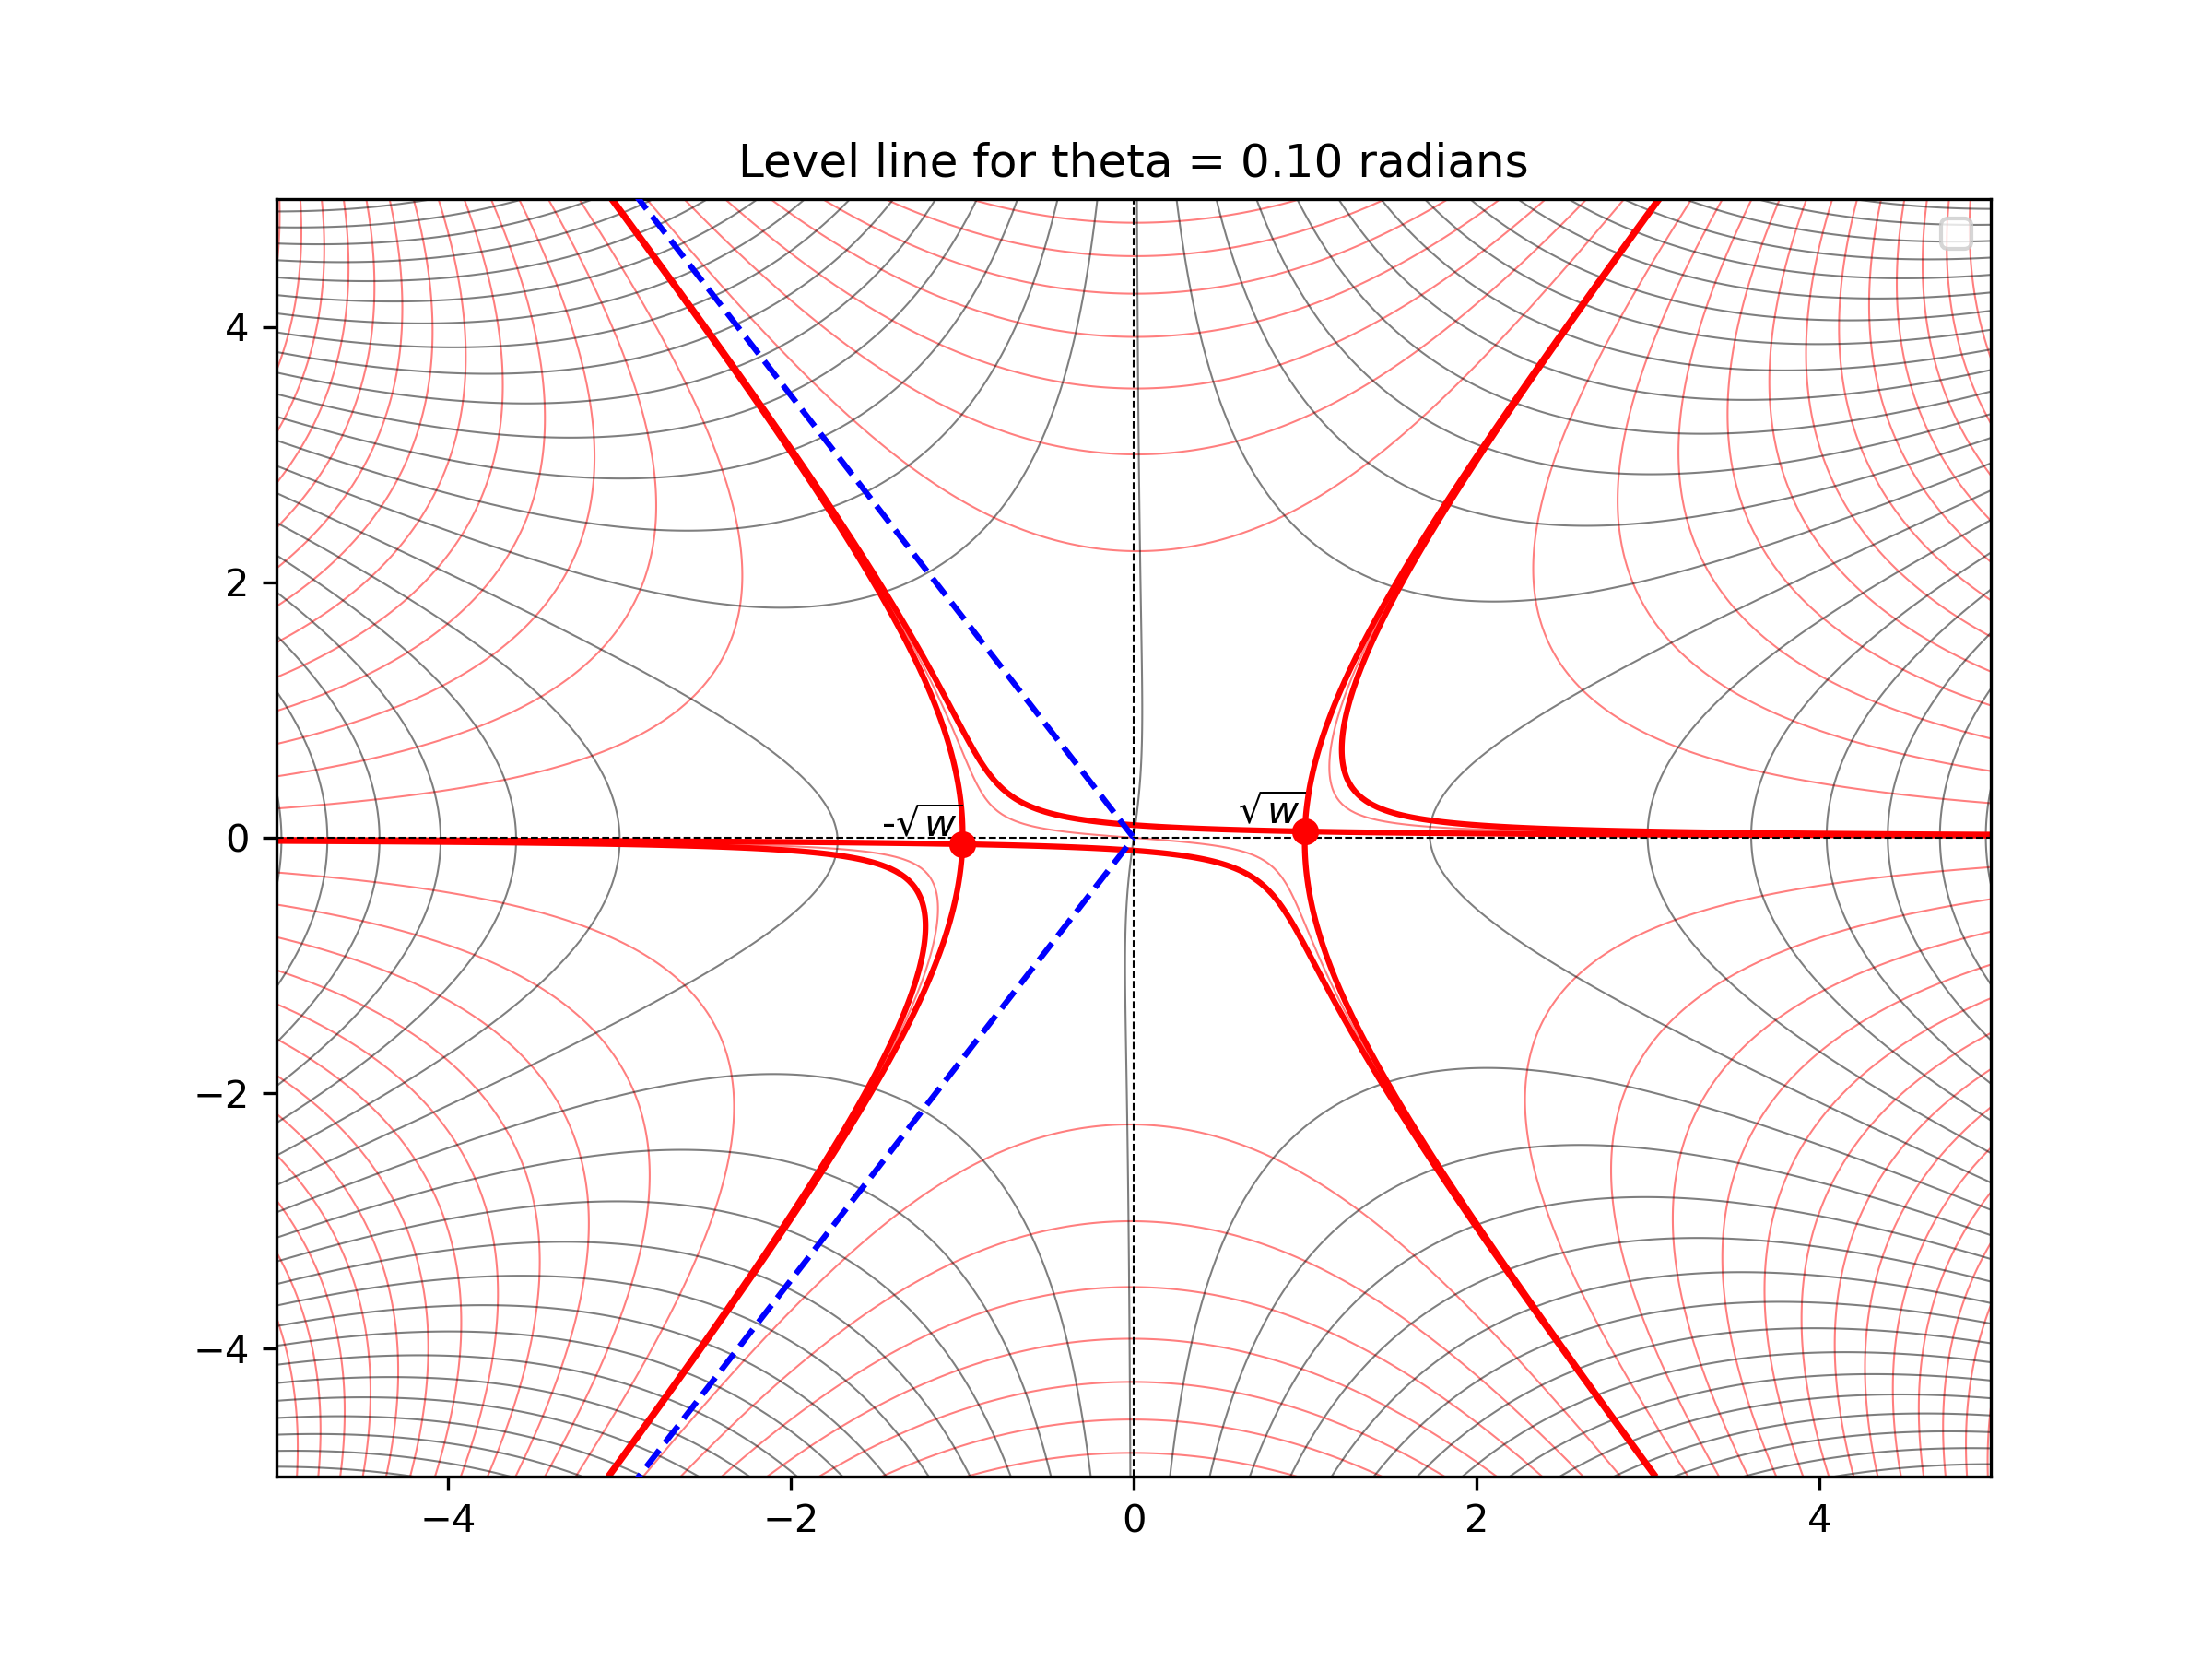
\includegraphics[width=0.49\textwidth]{/home/jvap/Documents/contour_plot_theta_0.10.png}}
	\subfigure{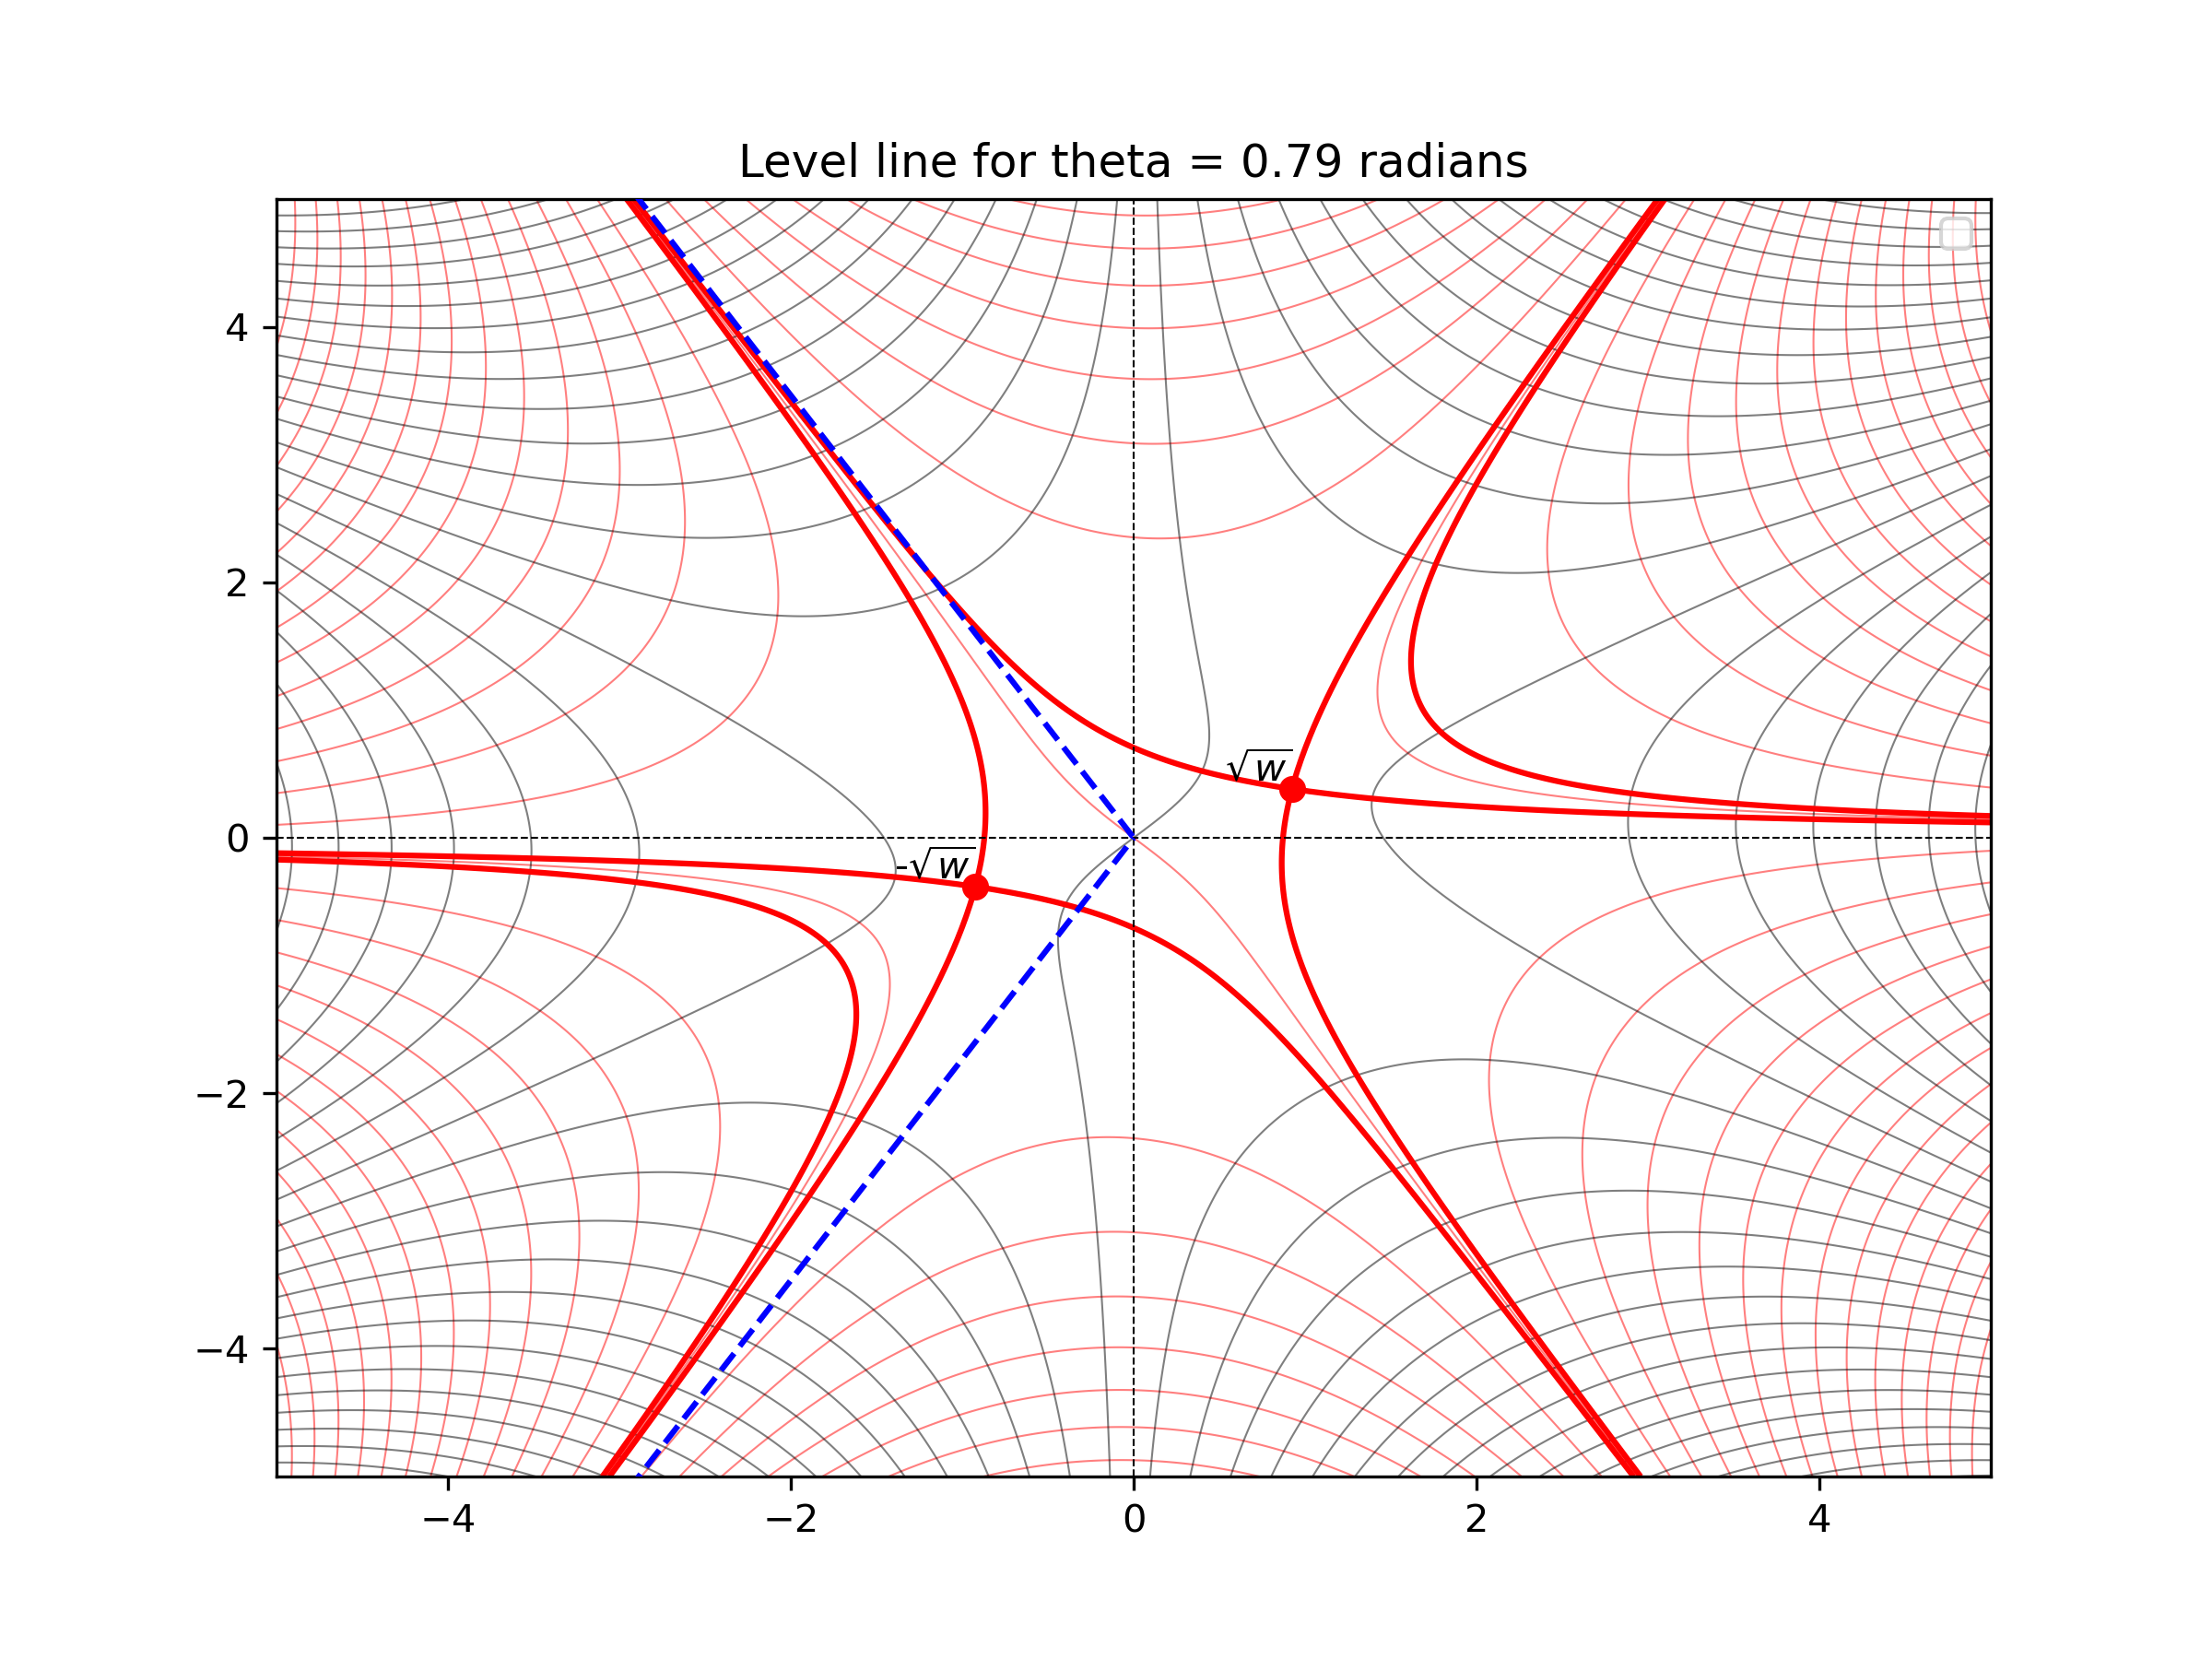
\includegraphics[width=0.49\textwidth]{/home/jvap/Documents/contour_plot_theta_0.79.png}}
	\subfigure{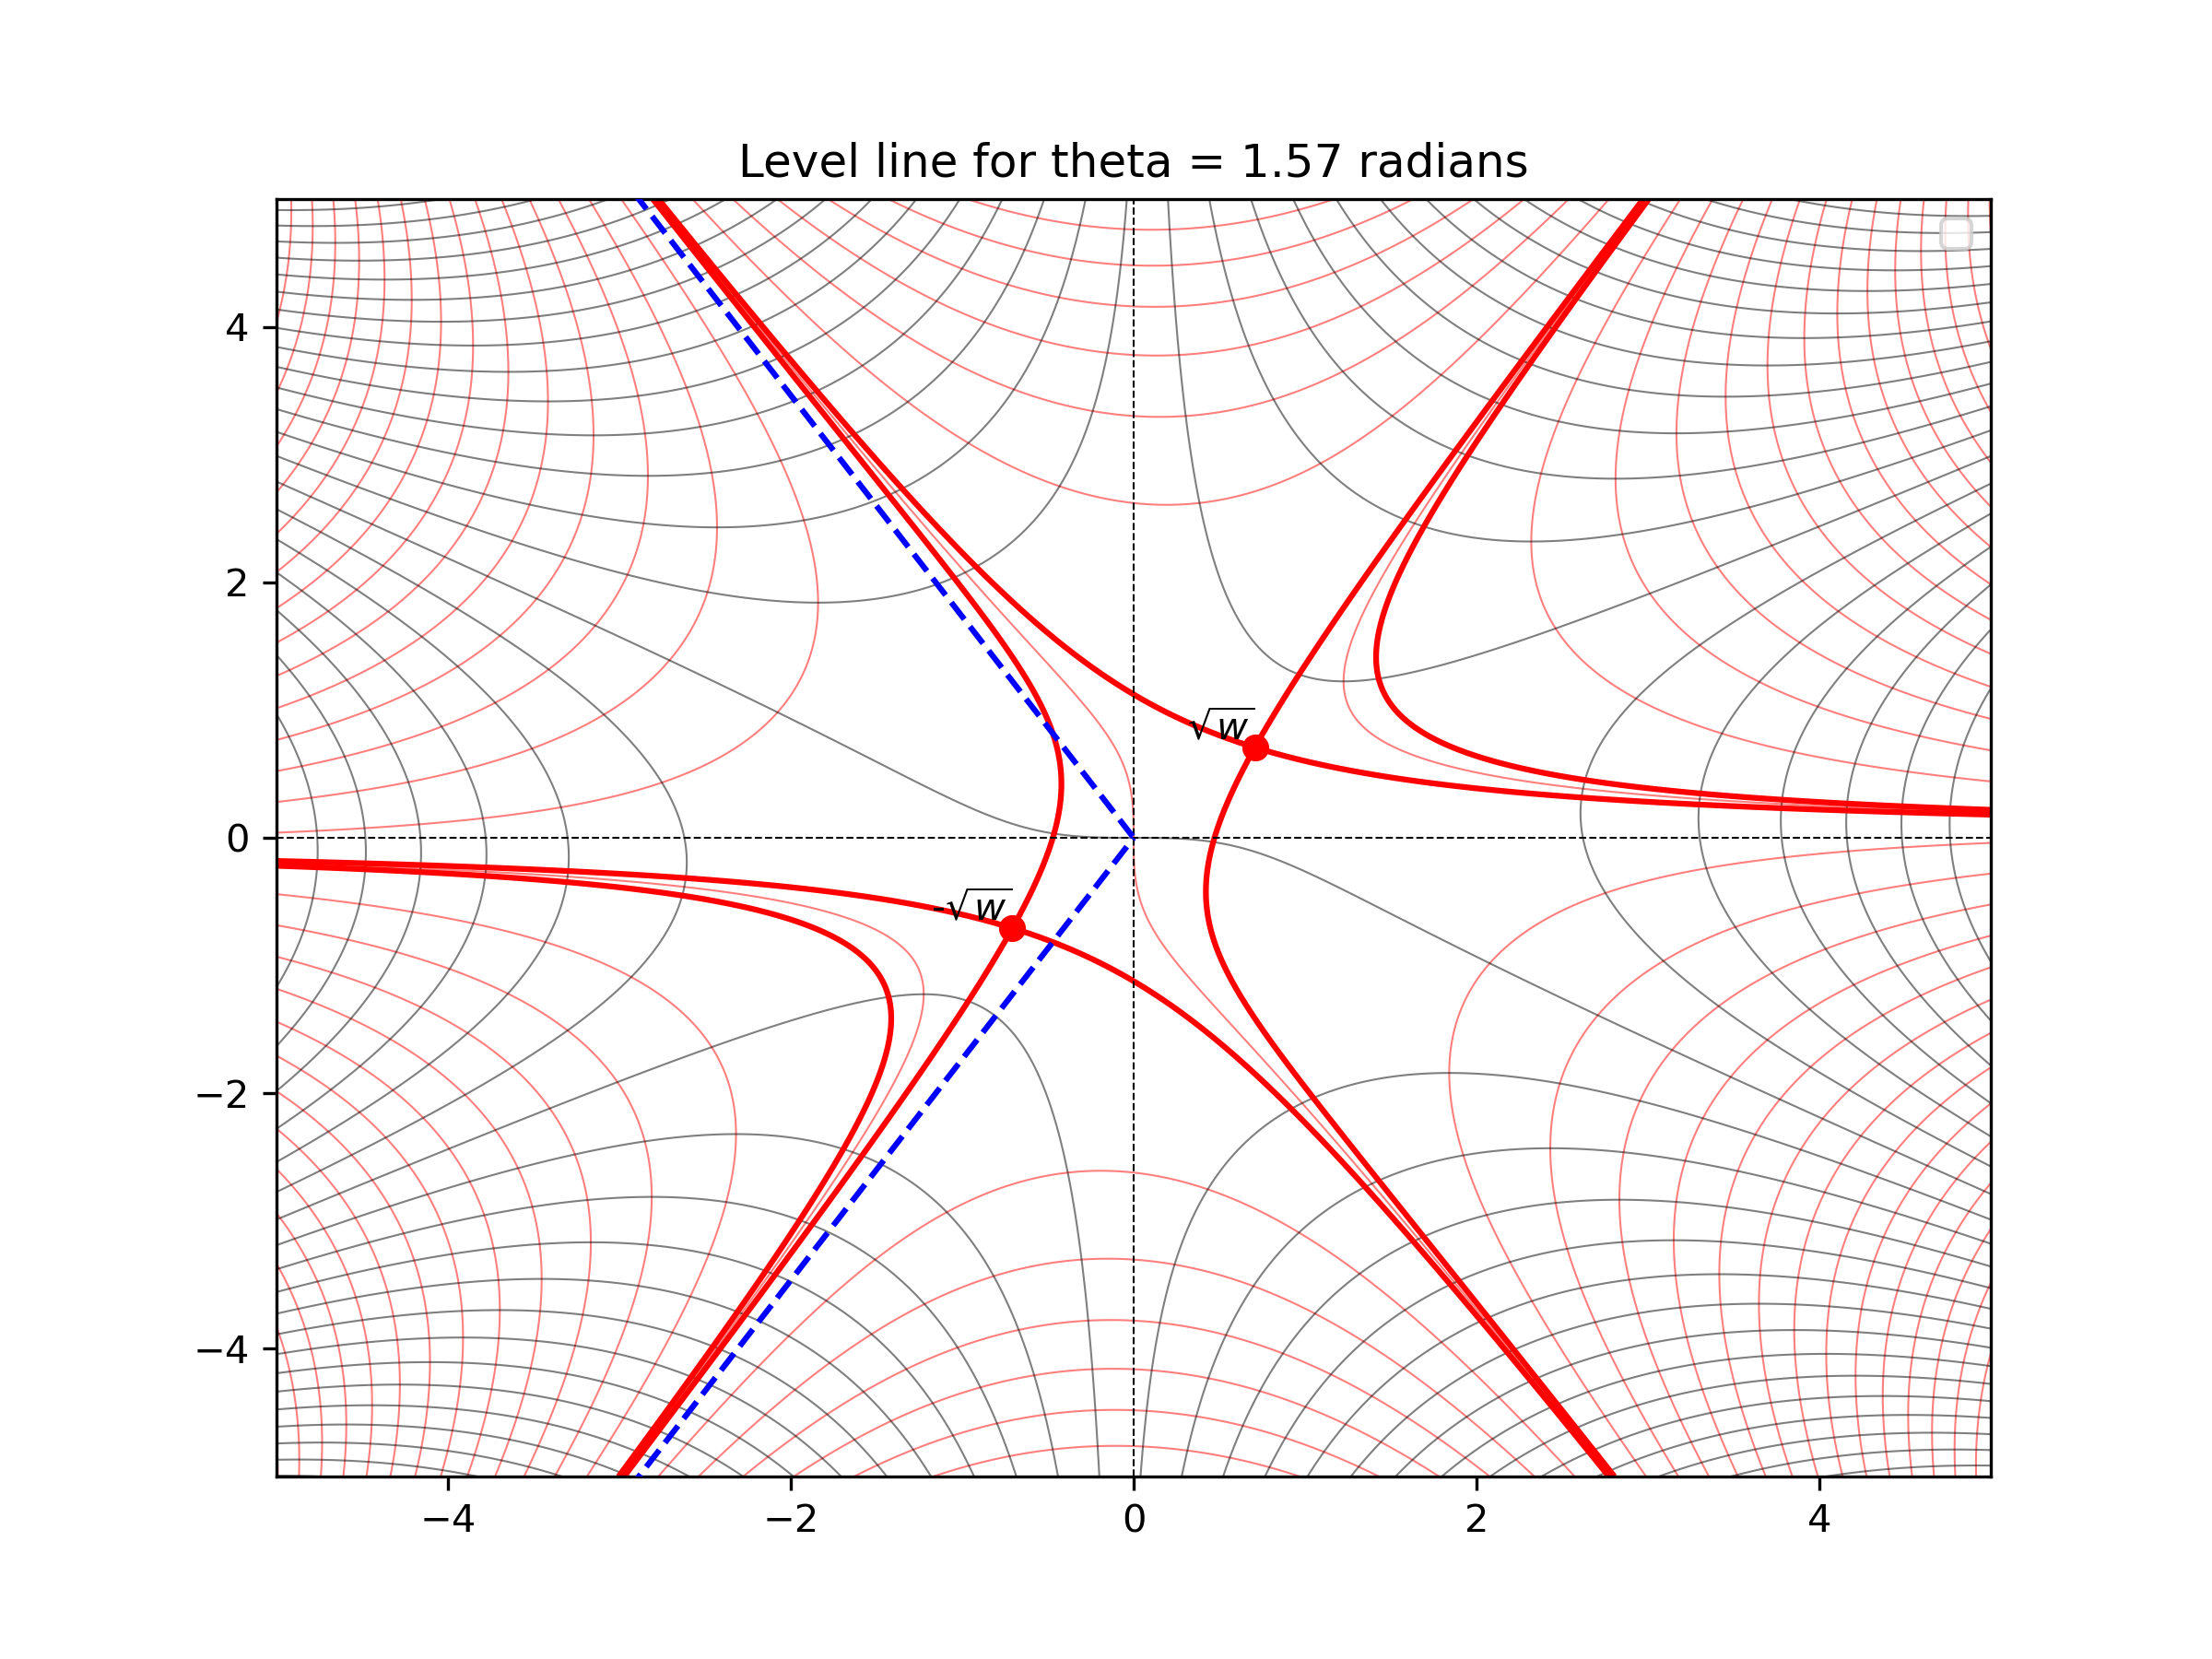
\includegraphics[width=0.49\textwidth]{/home/jvap/Documents/contour_plot_theta_1.57.png}}
	\subfigure{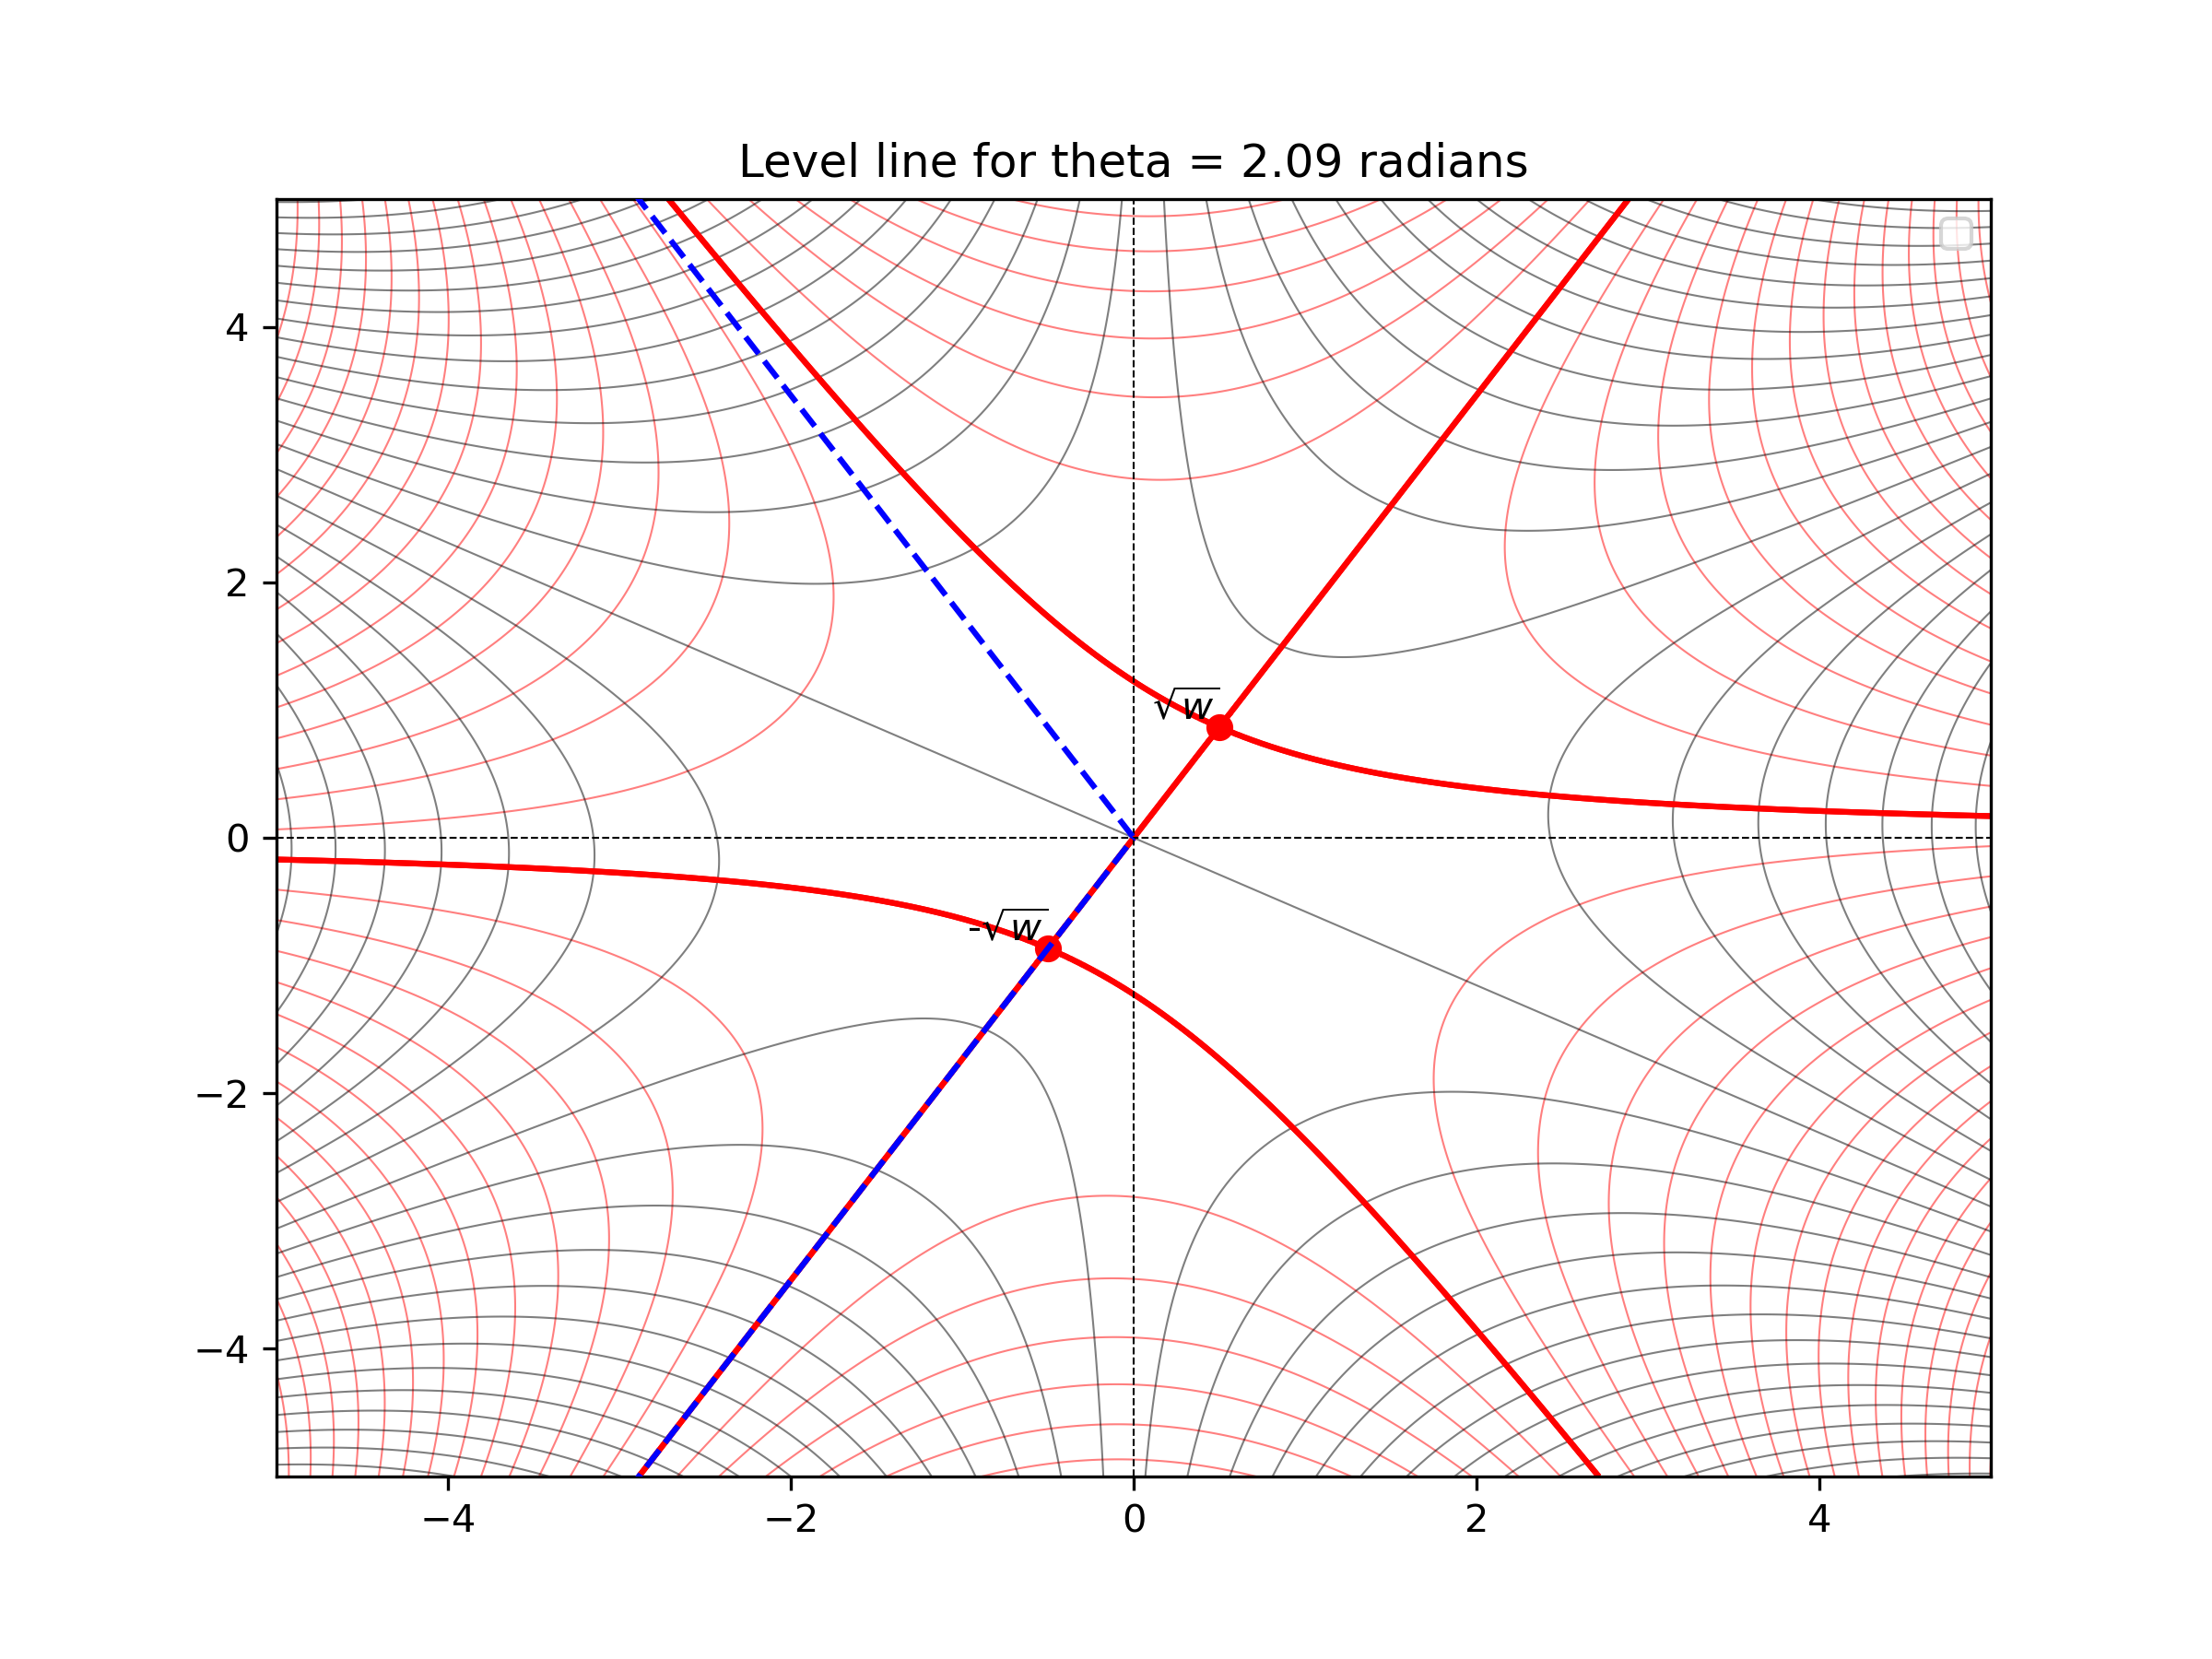
\includegraphics[width=0.49\textwidth]{/home/jvap/Documents/contour_plot_theta_2.09.png}}
	\subfigure{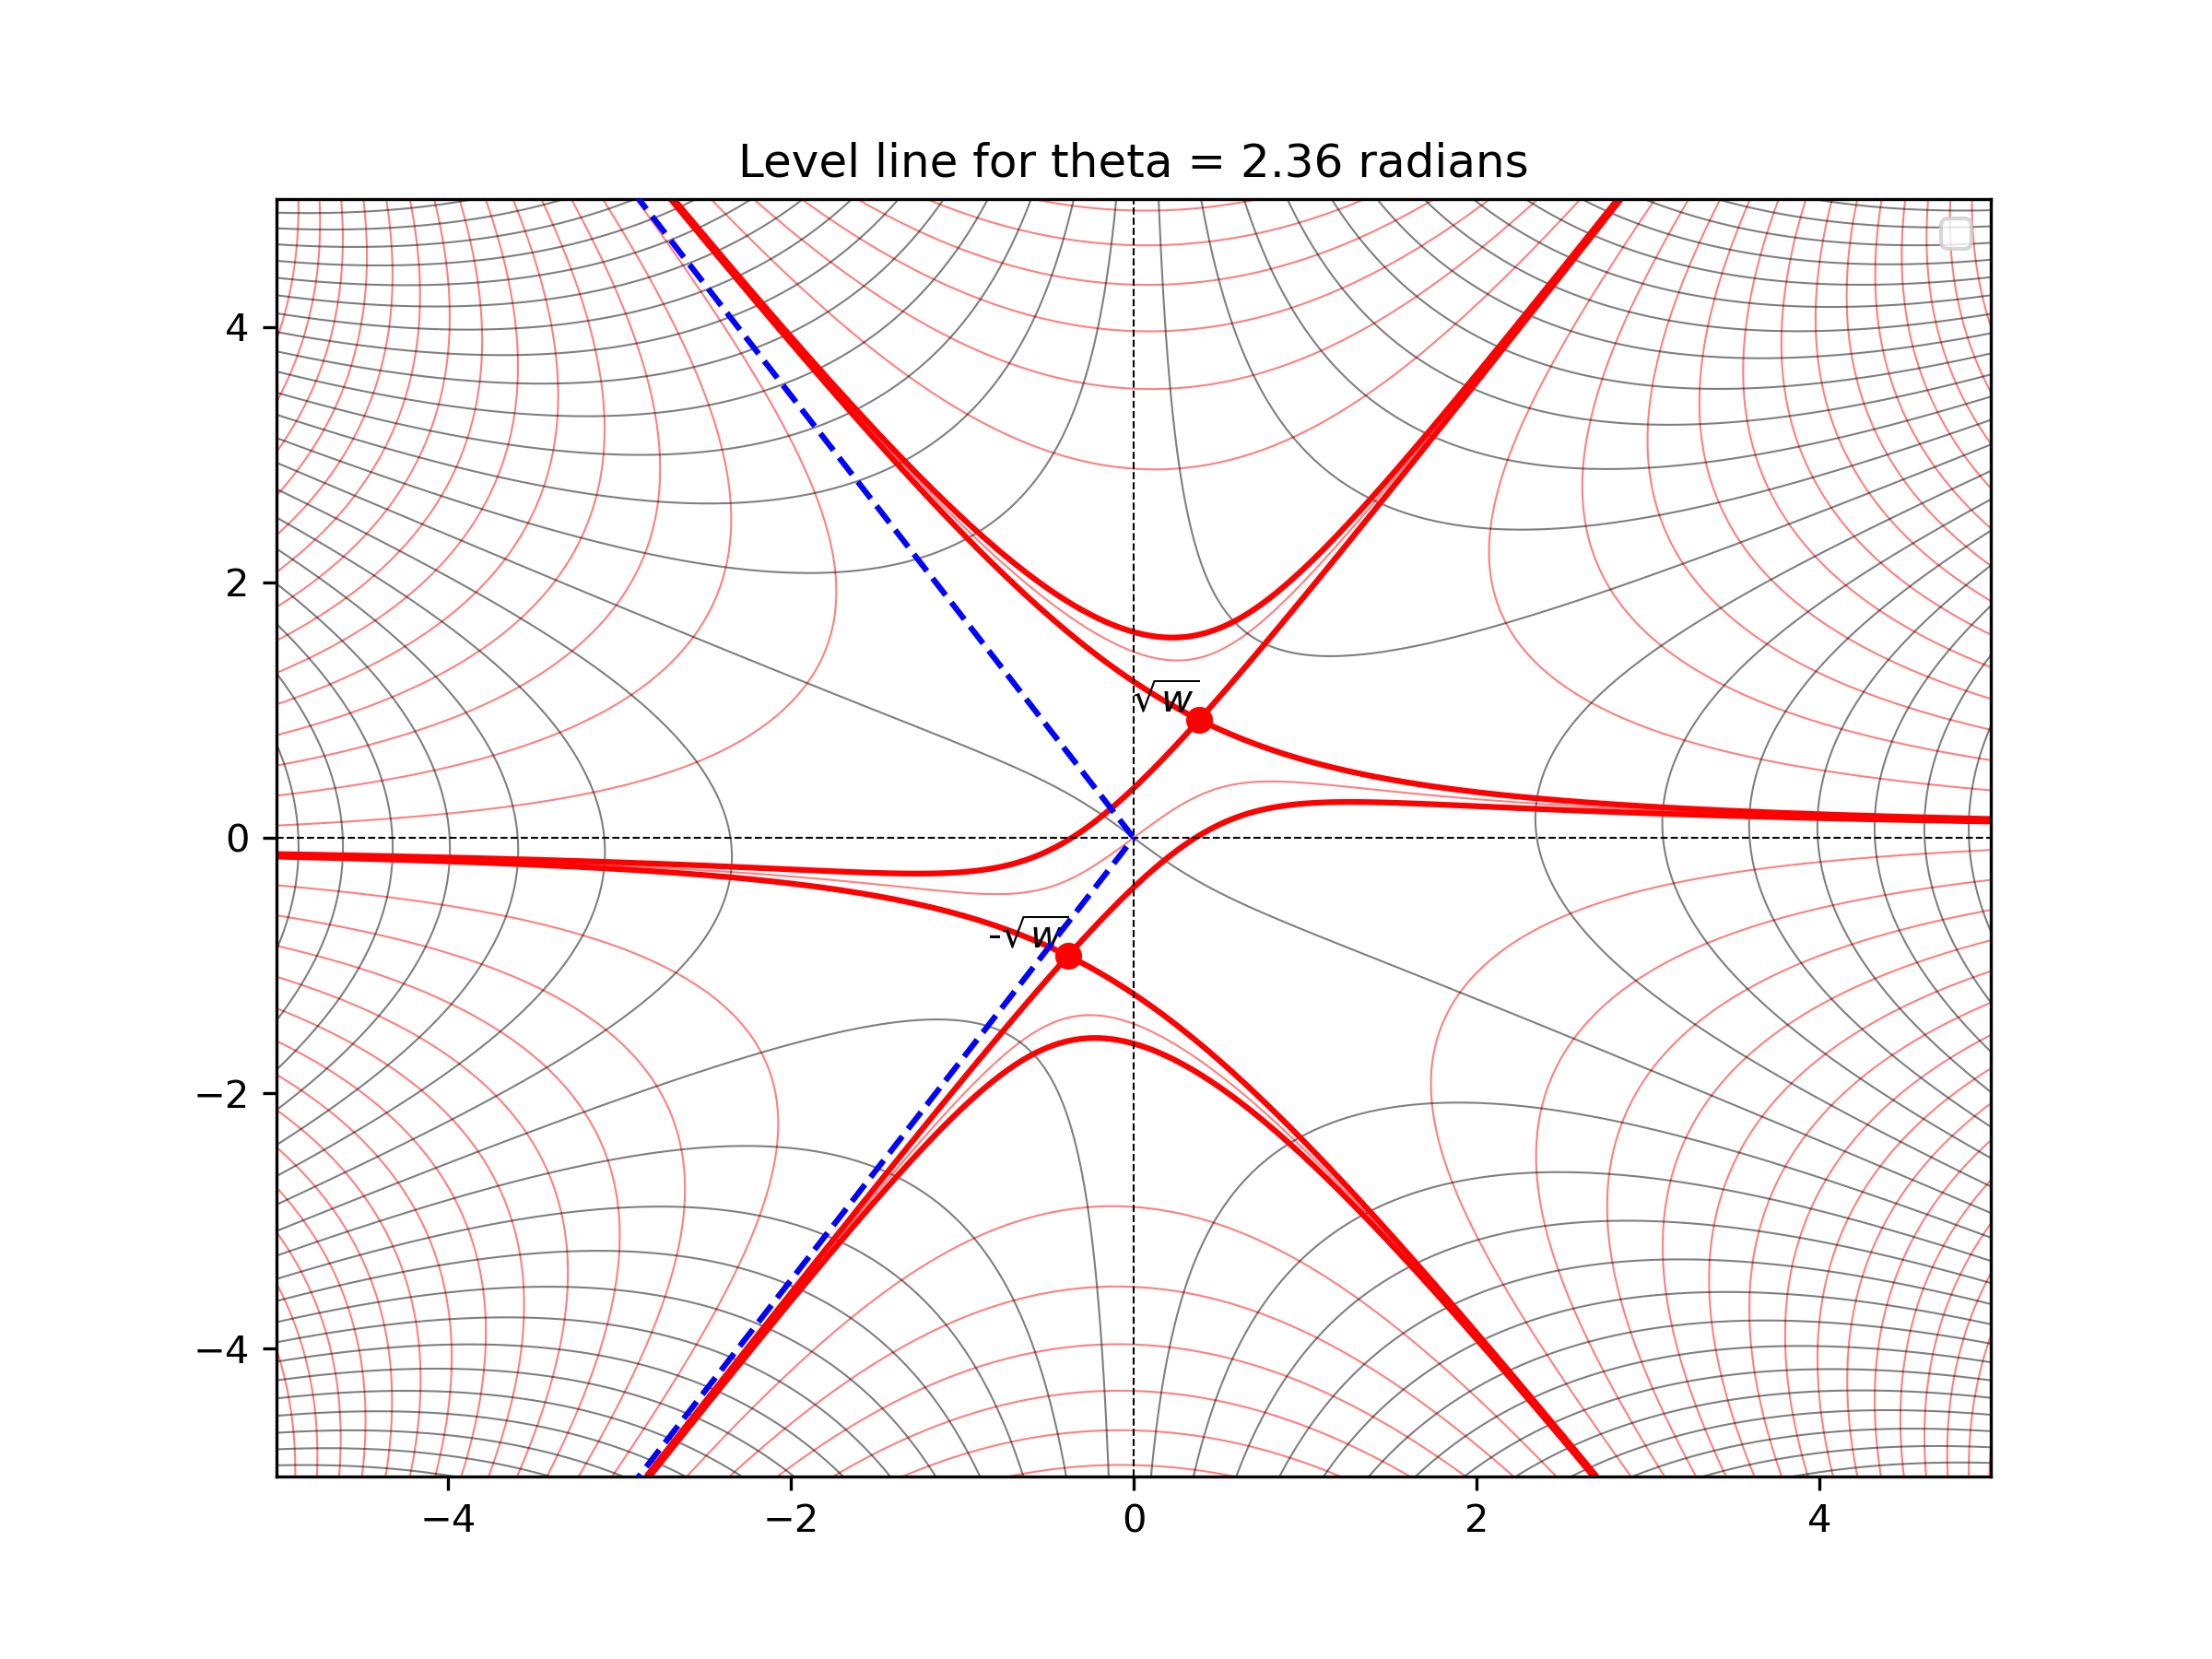
\includegraphics[width=0.49\textwidth]{/home/jvap/Documents/contour_plot_theta_2.36.png}}
	\subfigure{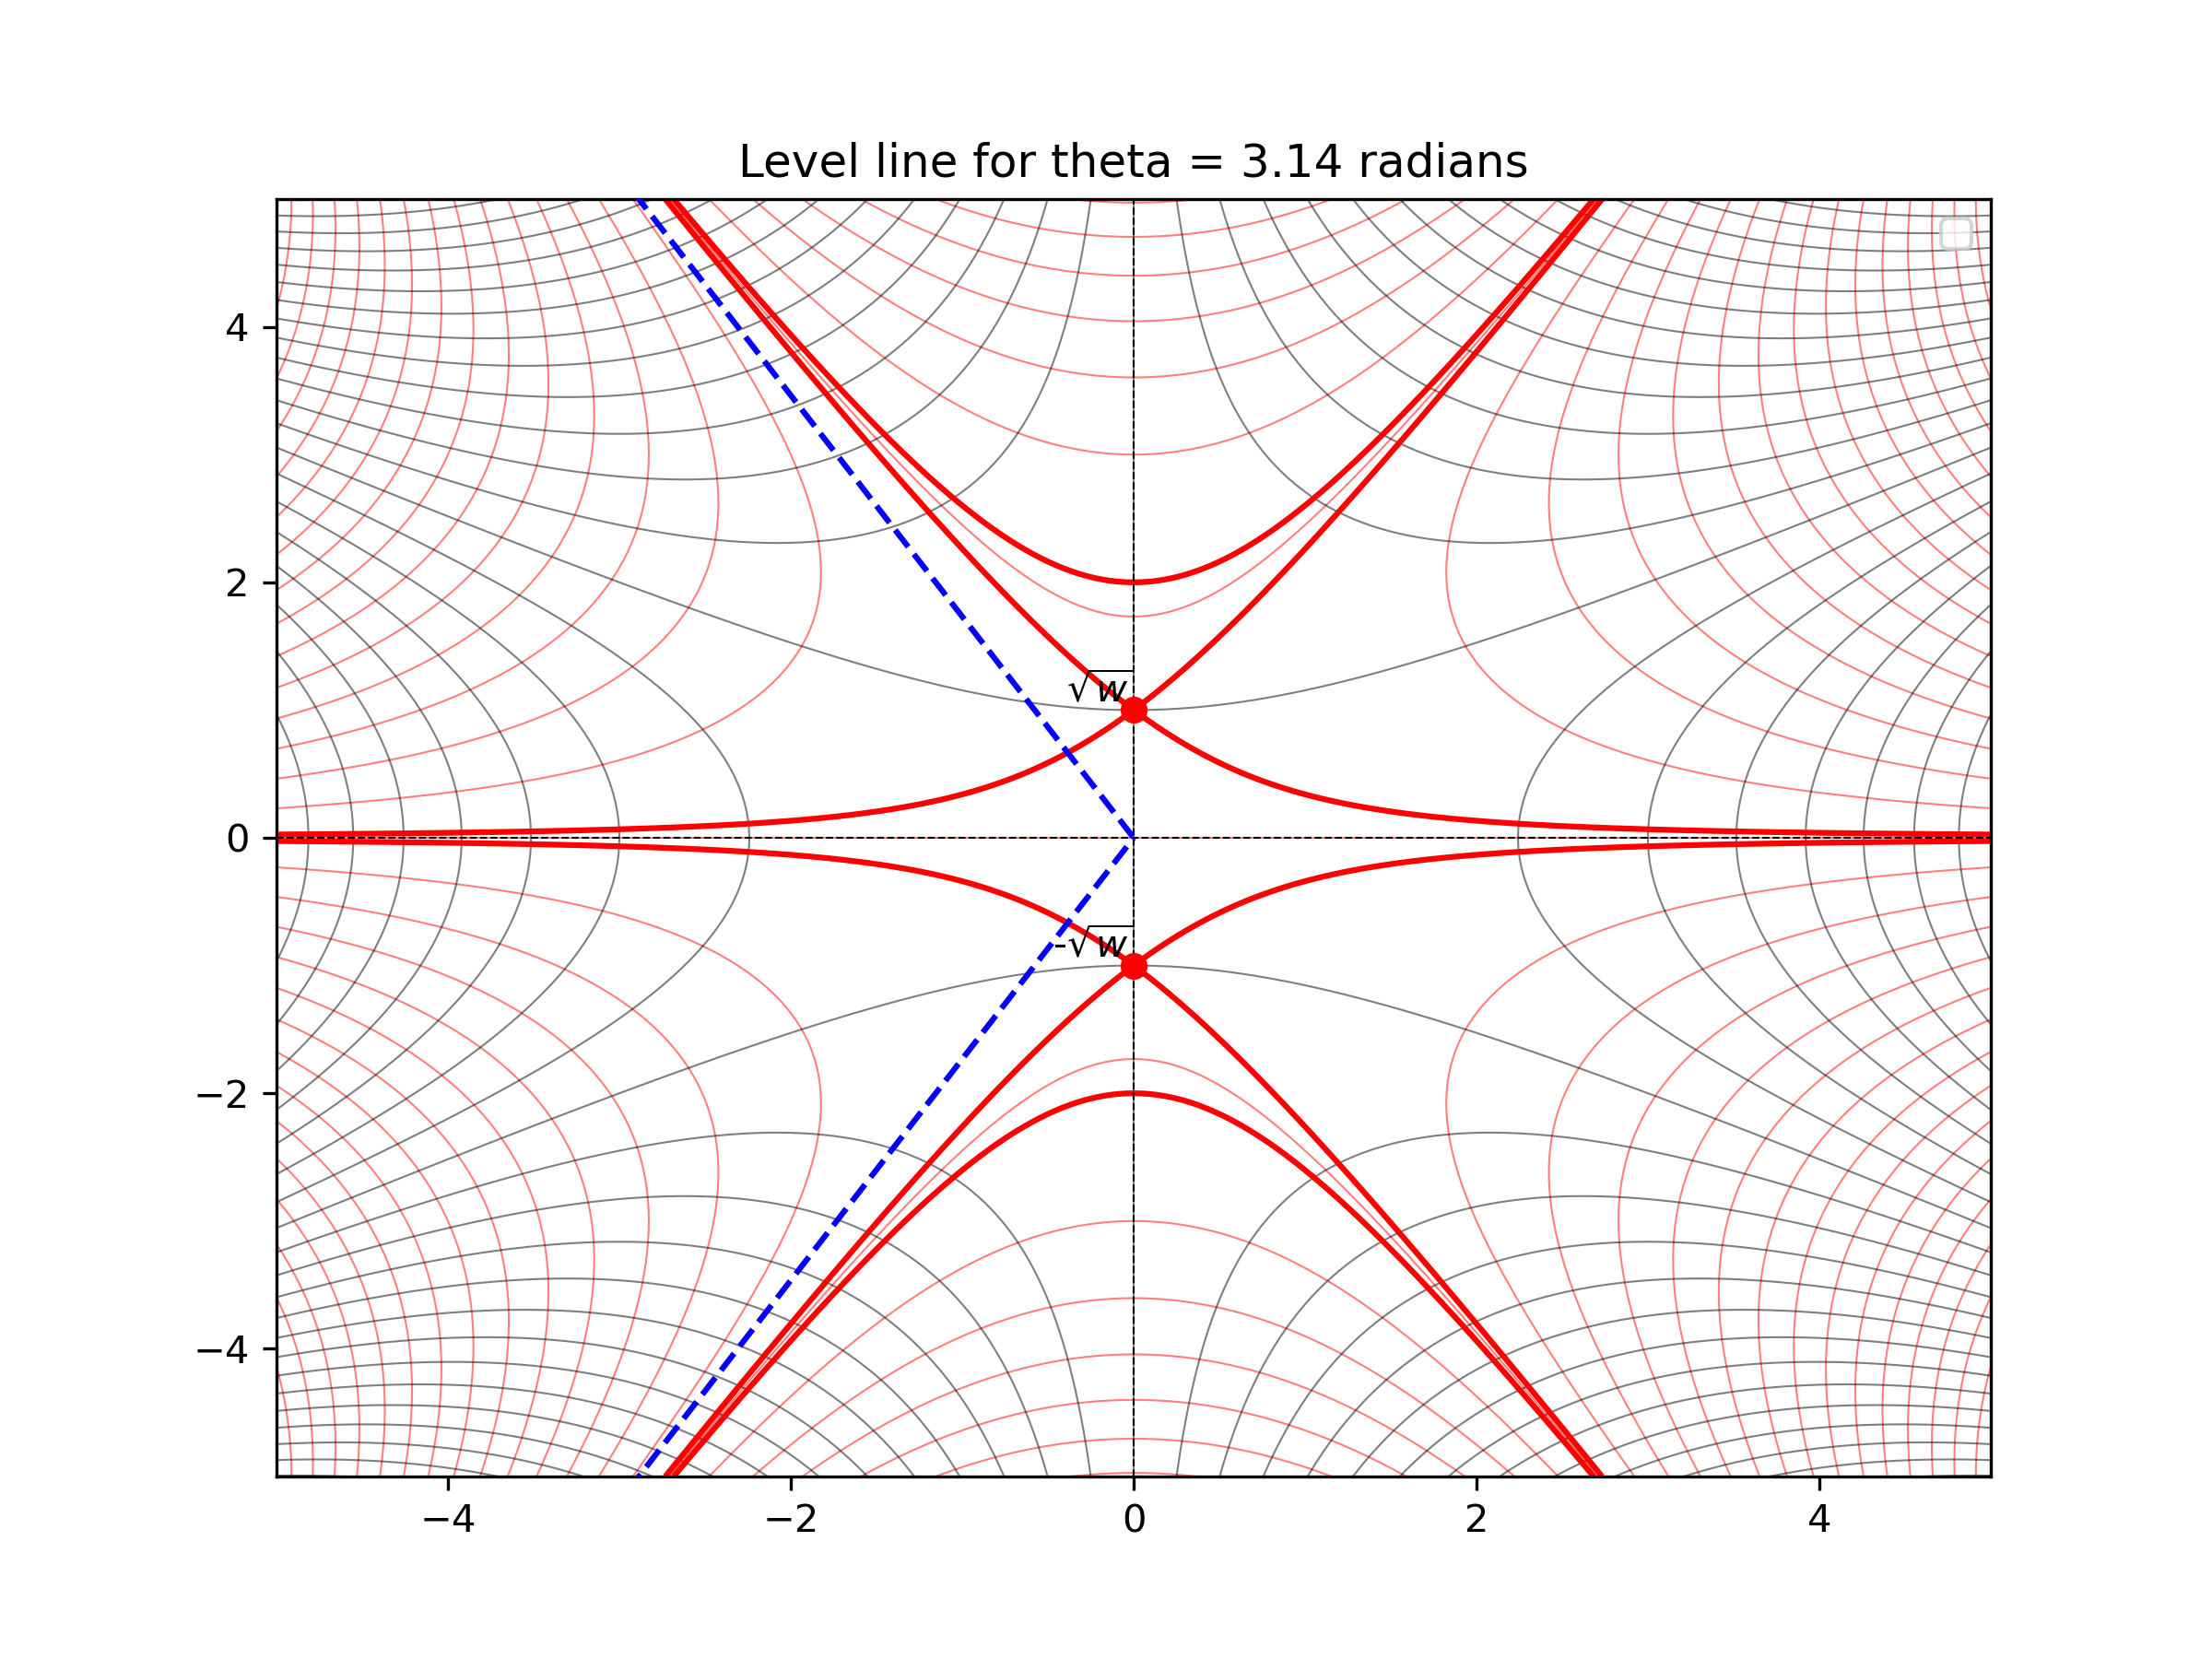
\includegraphics[width=0.49\textwidth]{/home/jvap/Documents/contour_plot_theta_3.14.png}}
	\caption{Scenarios for $\theta$}
	\label{Fig: theta cases}
\end{figure}

\subsubsection{Hermite's Polynomials}

For another example, let's explore the Hermite polynomial. We first note that such polynomials have an integral representation given by
\begin{equation}
	\begin{split}
		H_N(x) & \deff \frac{N!}{2\pi \ii} \int_{\Gamma} z^{-N-1} \ee^{2xz-z^2} \dd z \\
		& = \frac{N!}{2\pi \ii} \int_{\Gamma} \ee^{2xz-z^2 - (N+1)\log{(z)}} \dd z
	\end{split}
\end{equation}
Where $\Gamma$ is a contour that goeas around the origin coming and going from minus infinity such as $\Gamma = \{\lambda - \ii \delta : \lambda < 0 \} \cup \{\delta \ee^{\ii \theta}: -\pi/2 < \theta < \pi/2 \} \cup \{\lambda + \ii \delta : \lambda < 0 \}$. 
\begin{figure}[H]
	\centering
	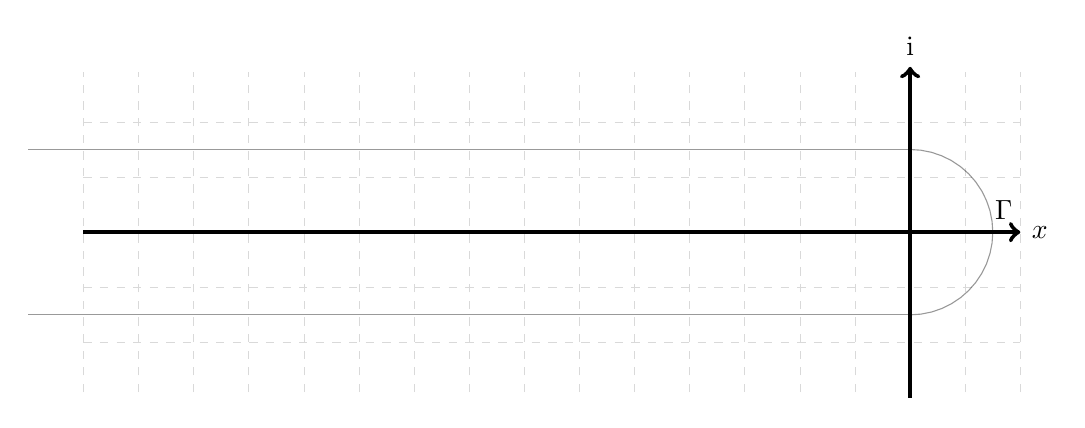
\begin{tikzpicture}[scale=.7]
		\draw[help lines, color=gray!30, dashed] (-15,-2.9) grid (2,2.9);
		\draw[->,ultra thick] (-15,0)--(2,0) node[right]{$x$};
		\draw[->,ultra thick] (0,-3)--(0,3) node[above]{$\ii$};
		
		\draw[opacity=0.4] plot[domain=-90:90] ({1.5*cos(\x)},{1.5*sin(\x)});
		\draw[opacity=0.4] plot[domain=-16:0] ({\x}, {1.5});
		\draw[opacity=0.4] plot[domain=-16:0] ({\x},{-1.5});
		
		\node (Gamma) at (1.7,0.4)    {$\Gamma$};
	\end{tikzpicture}
\end{figure}

Now, set $x \mapsto N^\alpha x$ and $z = N^\beta s$ and rewrite

\begin{equation*}
\begin{split}
		H_N(x) & = \frac{N! N^\beta}{2\pi \ii} \int_{\Gamma} \ee^{2(N^\alpha x)(N^\beta s)-(N^\beta s)^2 - (N+1)\log{(N^\beta s)}} \dd s \\
		& = \frac{N! N^\beta \ee^{-(N+1) \log{(N^\beta)}}}{2\pi \ii} \int_{\Gamma} \ee^{2(N^{\alpha+\beta} x s)-N^{2\beta} s^2 - (N+1)\log{(s)}} \dd s \\
		& \stackrel{(\alpha = \beta = 1/2)}{=} \frac{N! N^{\frac{1}{2}} N^{\frac{-(N+1)}{2}}}{2\pi \ii} \int_{\Gamma} \ee^{-N(-2 x s + s^2 + \log{(s)})} s^{-1} \dd s
\end{split}
\end{equation*}

We want to define $\Phi(s) \deff -2xs + s^2 + \log{(s)}$ such that we can calculate the critical points $t_c^\pm = \frac{x \pm \sqrt{x^2 - 2}}{2}$ where we divide three cases
\begin{enumerate}
	\item $s > \sqrt{2}$
	\item $0 < s < \sqrt{2}$	
	\item $s = \sqrt{2}$
\end{enumerate}
For the case $(1)$ we can see that the contribution for the asymptotic will come from $t_c^+$ while for case $(2)$ the contribution comes from both critical points, although depending on the real part one of the asymptotic may be exponential bigger than the other. The interesting case comes from $(3)$ where both critical point have the same value and $f''(t_c) = 0$. We need to rescale the variable somehow to get the behavior of the asymptotic. 

The idea is to perform a blow-up on the integral. We would have
$$\int_{\Gamma} \ee^{-N(-2 x t + t^2 + \log{(t)})} t^{-1} \dd t \deff \int_{\Gamma} \ee^{-N\Phi(t)} g(t) \dd t $$
where we know $\Phi$ to have first and second derivative equal to zero at $t_c = \sqrt{2}/2$. First we need to divide the integral in three parts
$$ \int_{\Gamma_1} \ee^{-N\Phi(t)} g(t) \dd t + \int_{t_c - \delta}^{t_c + \delta} \ee^{-N\Phi(t)} g(t) \dd t + \int_{\Gamma_2} \ee^{-N\Phi(t)} g(t) \dd t \approx \int_{t_c - \delta}^{t_c + \delta} \ee^{-N\Phi(t)} g(t) \dd t$$
 So we would write
$$\Phi(t) = \frac{\Phi^{(3)}(t_c)}{3!} t^3 + \Boh(t^4).$$
We now want to find a change of variable $\Phi(t) = s^3$ such that $s^3 = \Phi(t) = \tilde{\Phi}(t) t^2$. If we have such an equality we know $\tilde{\Phi}$ to be analytic, $\tilde{\Phi}'(t_c) \neq 0$ and $\tilde{\Phi}(t) = \frac{\Phi^{(3)}(t_c)}{3!} t + \Boh{(t^2)} \deff c_0 t + \Boh{(t^2)}$. 

To find such a change of variable we need to investigate the function
$$H(t, s) = t^2 \tilde{\Phi}(t) - s^3.$$
We first note that we can not find apply the Inverse Function Theorem in such a function because it's derivative is zero at $(t_c, 0)$. For that we introduce a new variable function $v = v(t)$ such that $t = v s$. Now,
$$ H(t, s) = s^3 \left( \frac{v^2}{s} \tilde{\Phi}(vs) -1 \right) \deff s^3 Q(v, s) .$$
We can of course also write $\partial_s Q(v, s) = v' \partial_v Q + \partial_s Q = 0$ giving us
$$ \frac{\partial v(t)}{\partial s} = - \frac{\partial_s Q}{\partial_v Q}.$$
It remains to check that we can indeed apply the Implicit Function Theorem to this function $Q$. For that we compute teh derivative of the function. As
$$Q(s, v(s)) = -1 + \frac{v^2}{s} (c_0 vs + \Boh(v^2s^2)) = -1 + c_0v^3 + \Boh(v^4s)$$
and because of that
$$\partial_v Q = 3 c_0 v^2 + \Boh{(v^3s)} \neq 0, \ \ \text{if} \ \ v(t_c) \neq 0.$$

Because of the theorem we can say that there exists a function $v(t)$ such that $H(vs, s) = 0$ and $v(t_c) = v_0$. Getting back to the integral we use $t = vs$ to write
\begin{equation}
	\begin{split}
		& = \int_{\alpha}^{\beta} \ee^{-Ns^3} (v(s) + v'(s)s) g(v(s)s) \dd s, \ \ \alpha = - \sqrt[3]{\Phi(\delta - t_c)} \ \ \text{and} \ \ \beta = \sqrt[3]{\Phi(\delta + t_c)} \\
		&  = \int_{\alpha}^{\beta} \ee^{-Ns^3} \frac{(v(s) + v'(s)s)}{v(s) s} \dd s \\
		& = \int_{\alpha}^{\beta} \ee^{-Ns^3} \left( \frac{1}{s} + \frac{v'(s)}{v(s)} \right) \dd s
	\end{split}
\end{equation}
where hopefully I can apply Laplace.

 
\begin{figure}[h] 
	\centering
	\subfigure{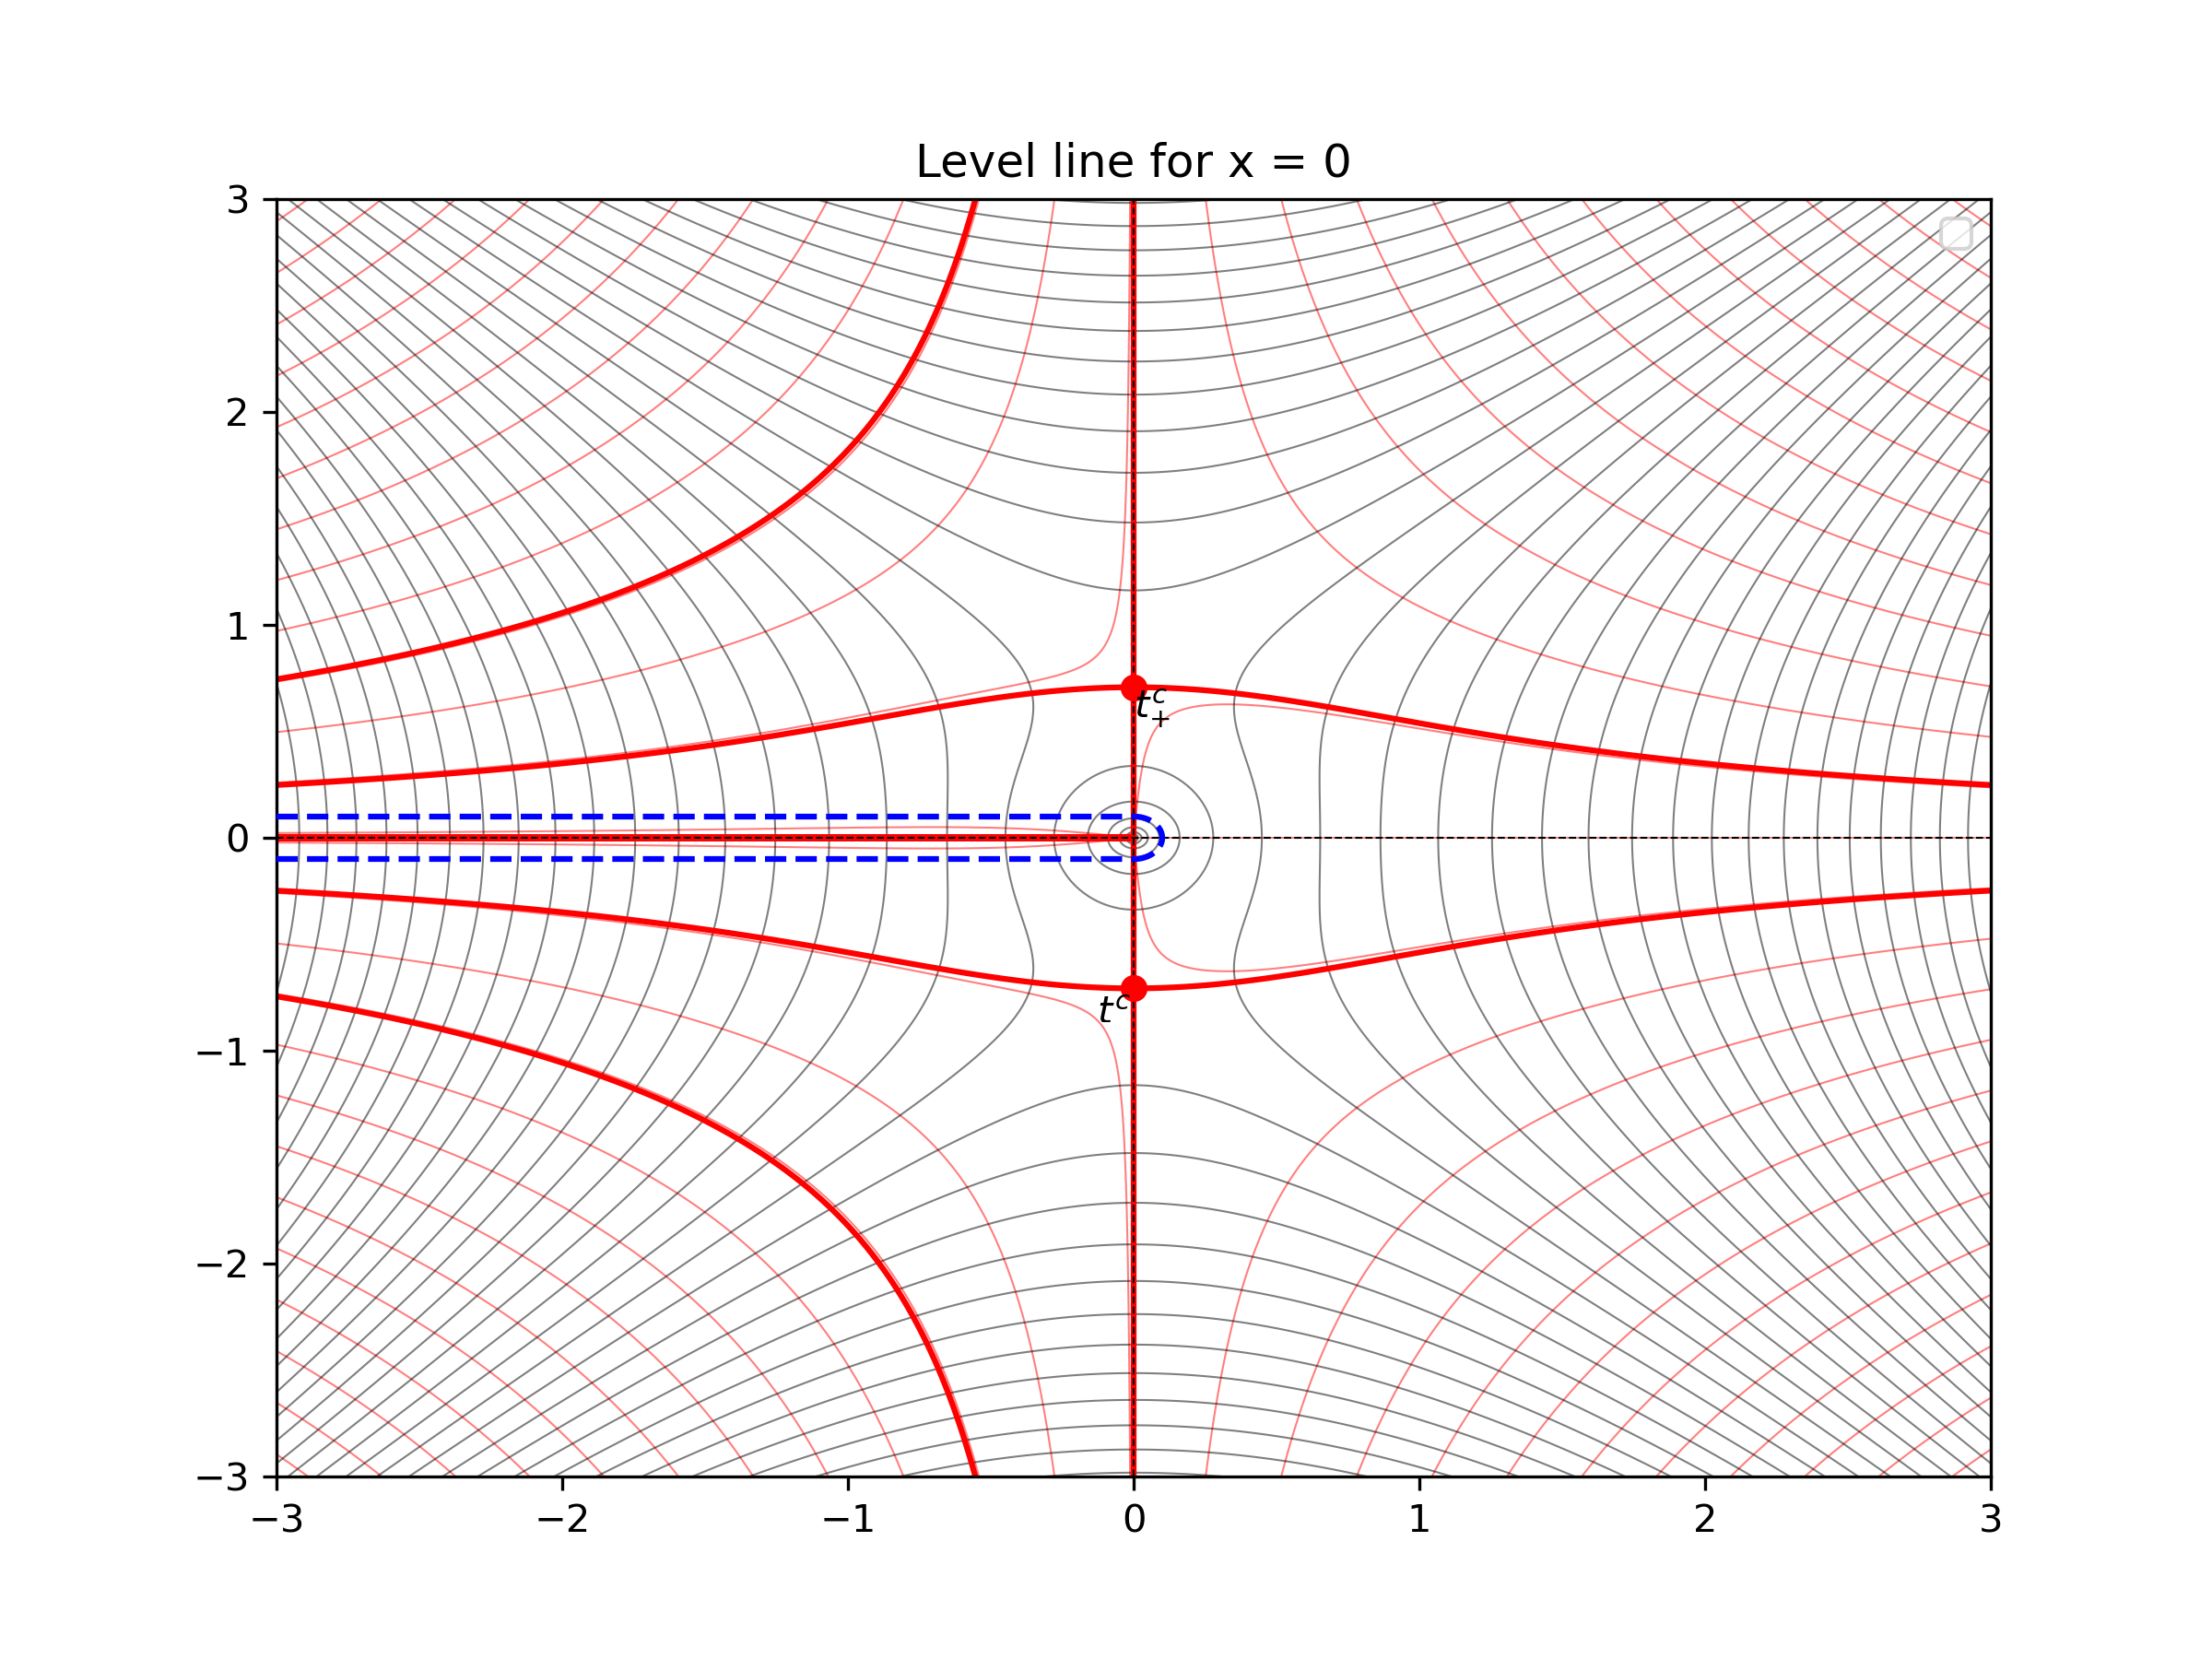
\includegraphics[width=0.49\textwidth]{/home/jvap/Documents/g-contour_plot_theta_0.png}}
	\subfigure{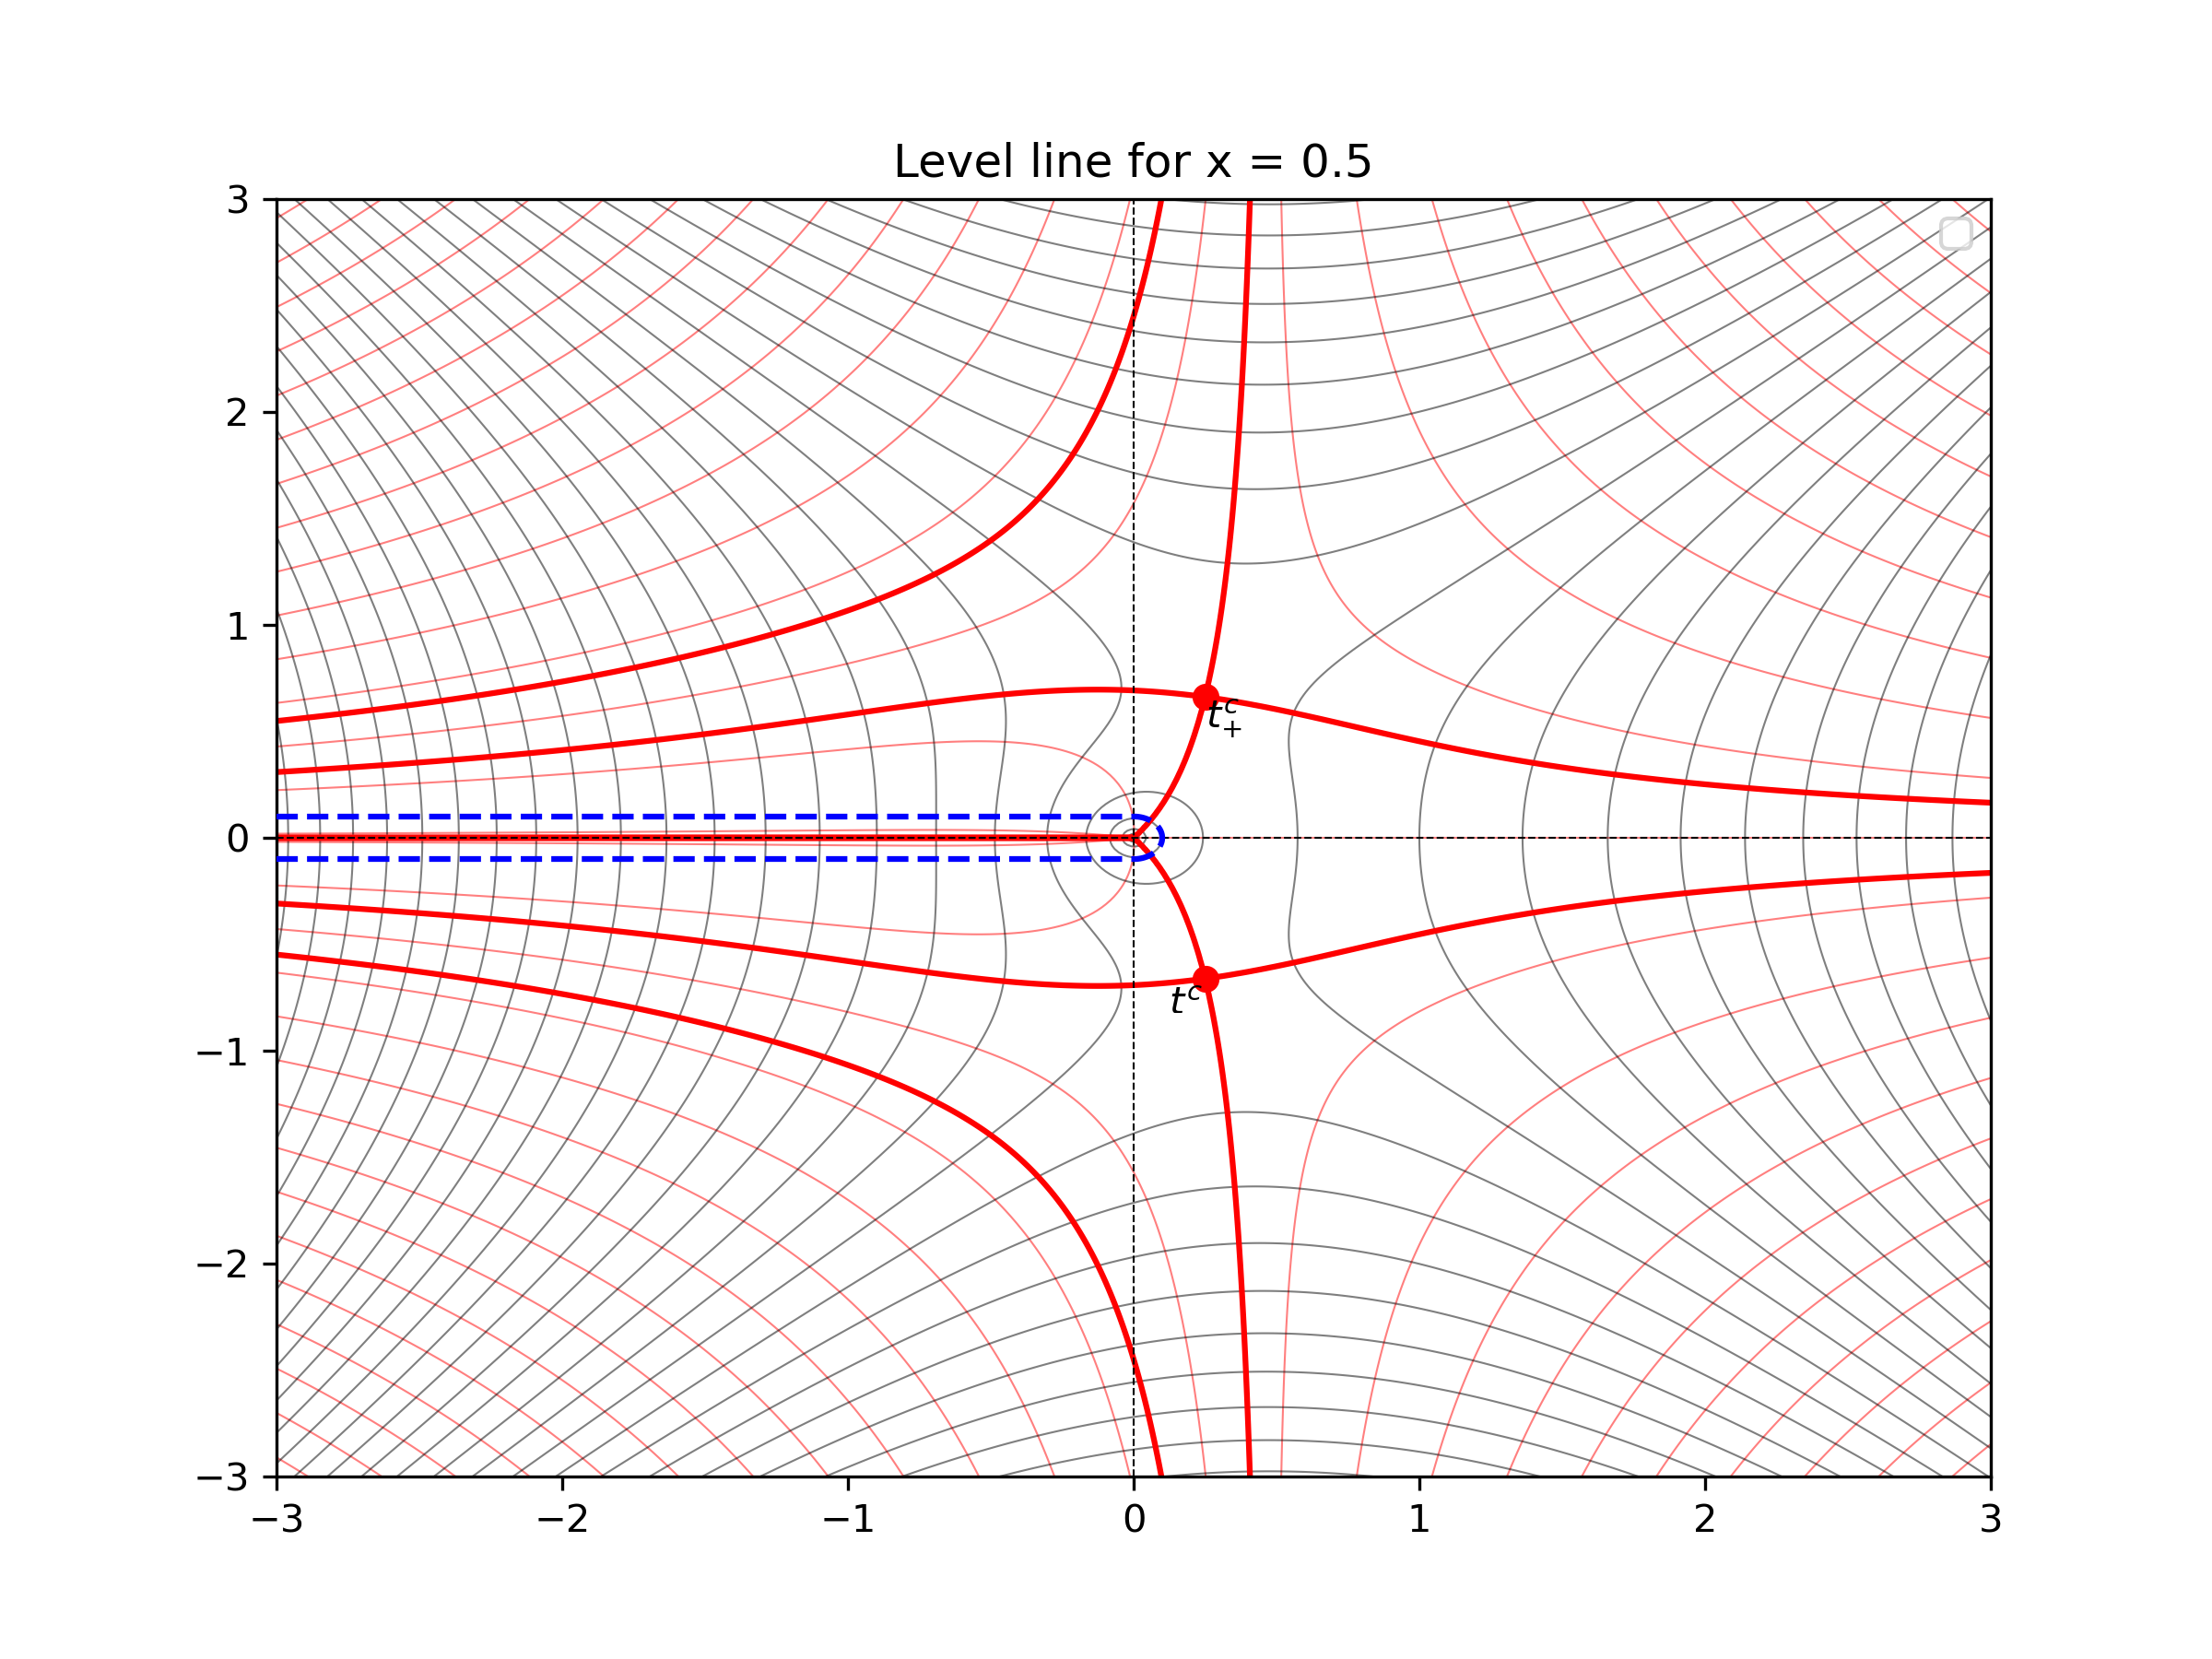
\includegraphics[width=0.49\textwidth]{/home/jvap/Documents/g-contour_plot_theta_0.5.png}}
	\subfigure{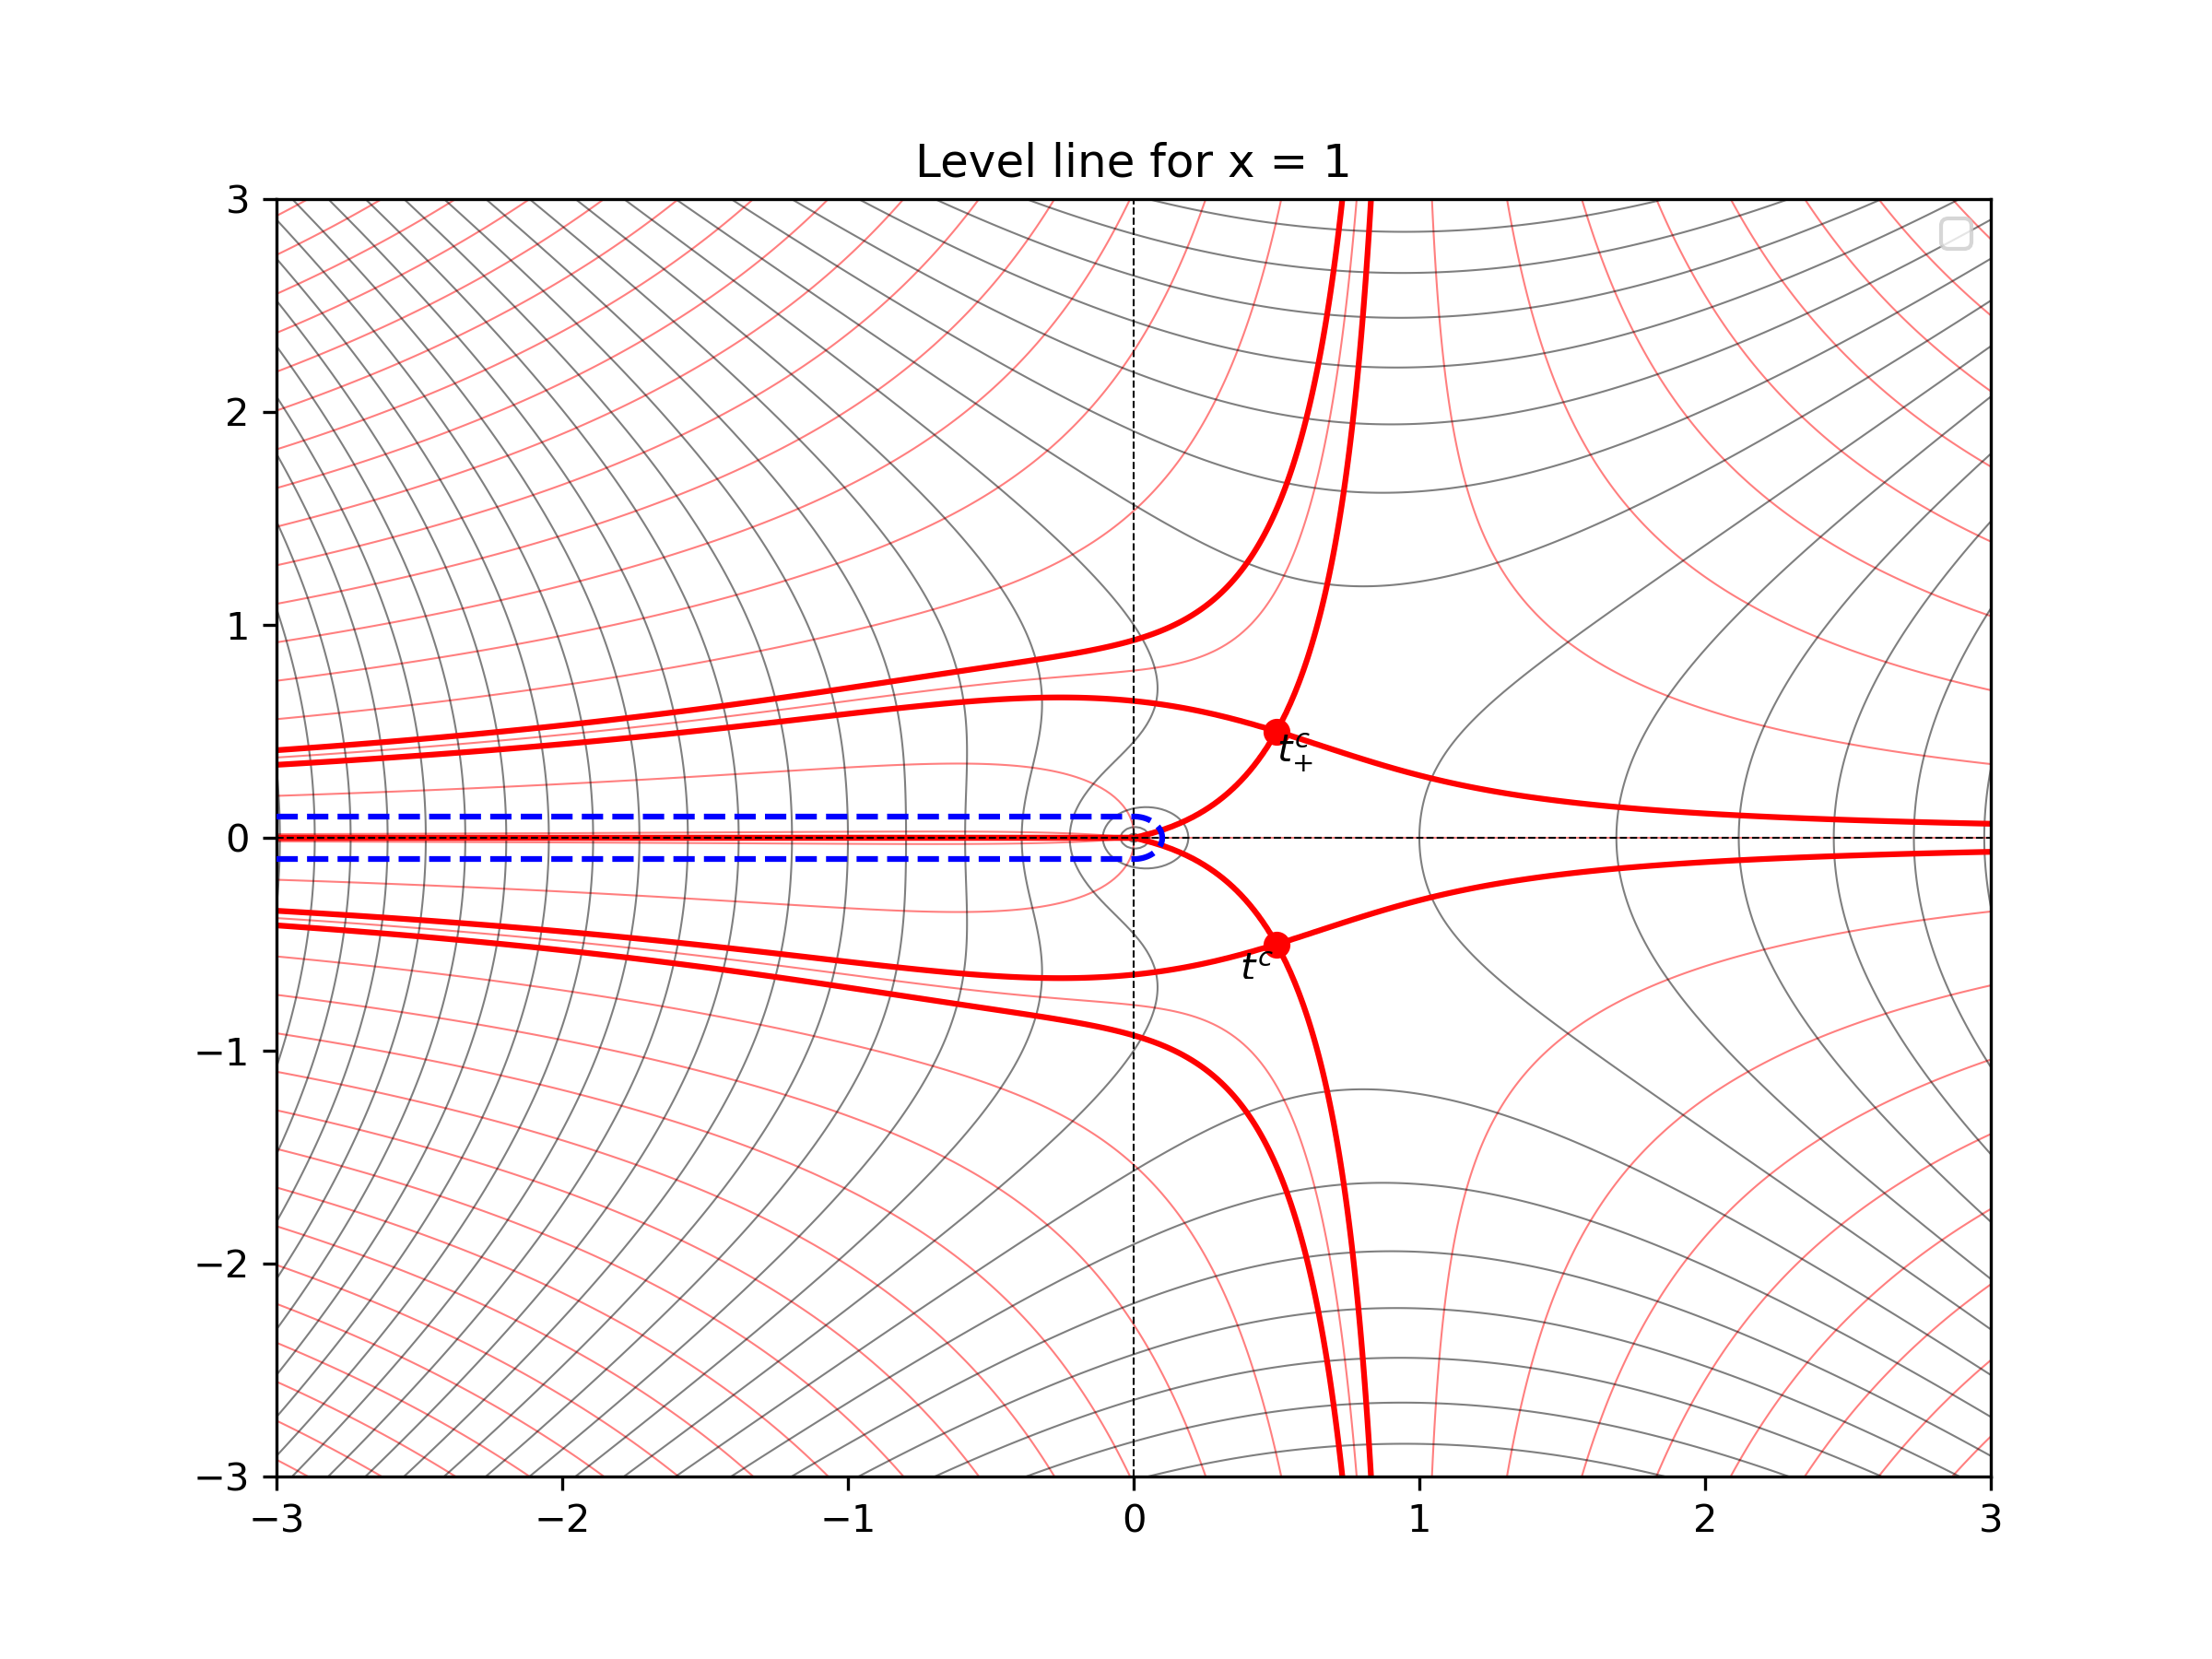
\includegraphics[width=0.49\textwidth]{/home/jvap/Documents/g-contour_plot_theta_1.png}}
	\subfigure{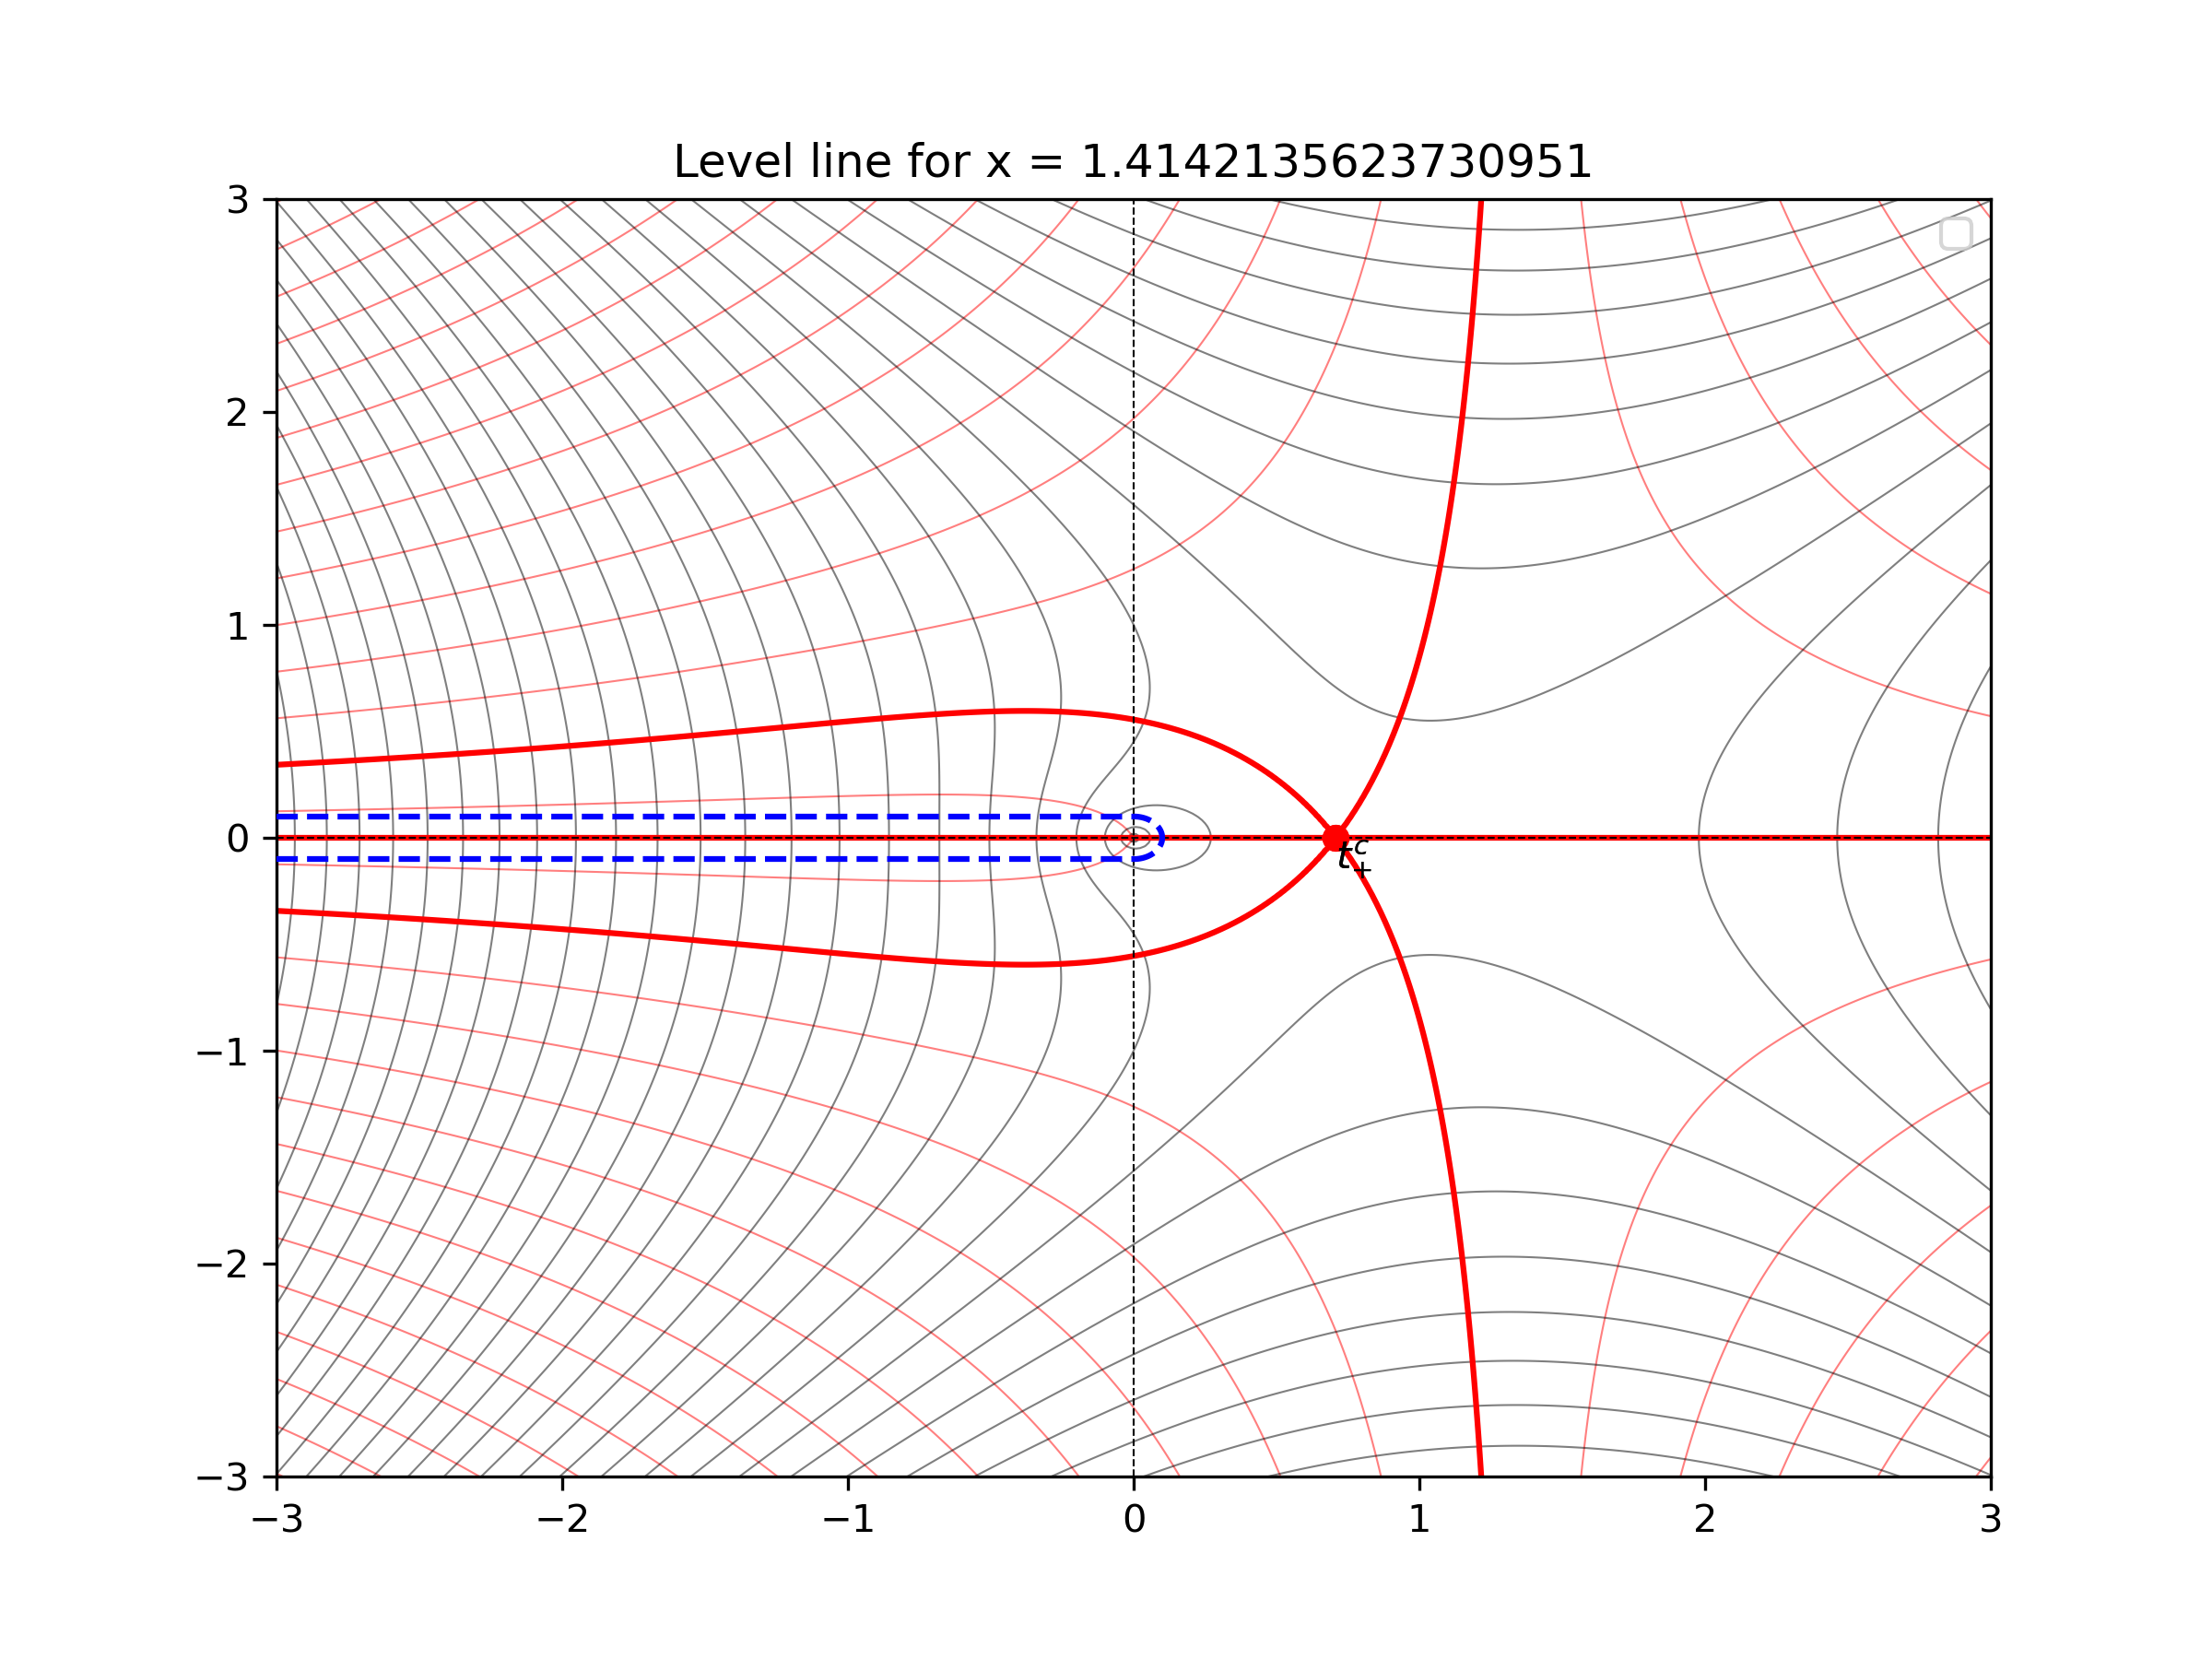
\includegraphics[width=0.49\textwidth]{/home/jvap/Documents/g-contour_plot_theta_1.4.png}}
	\subfigure{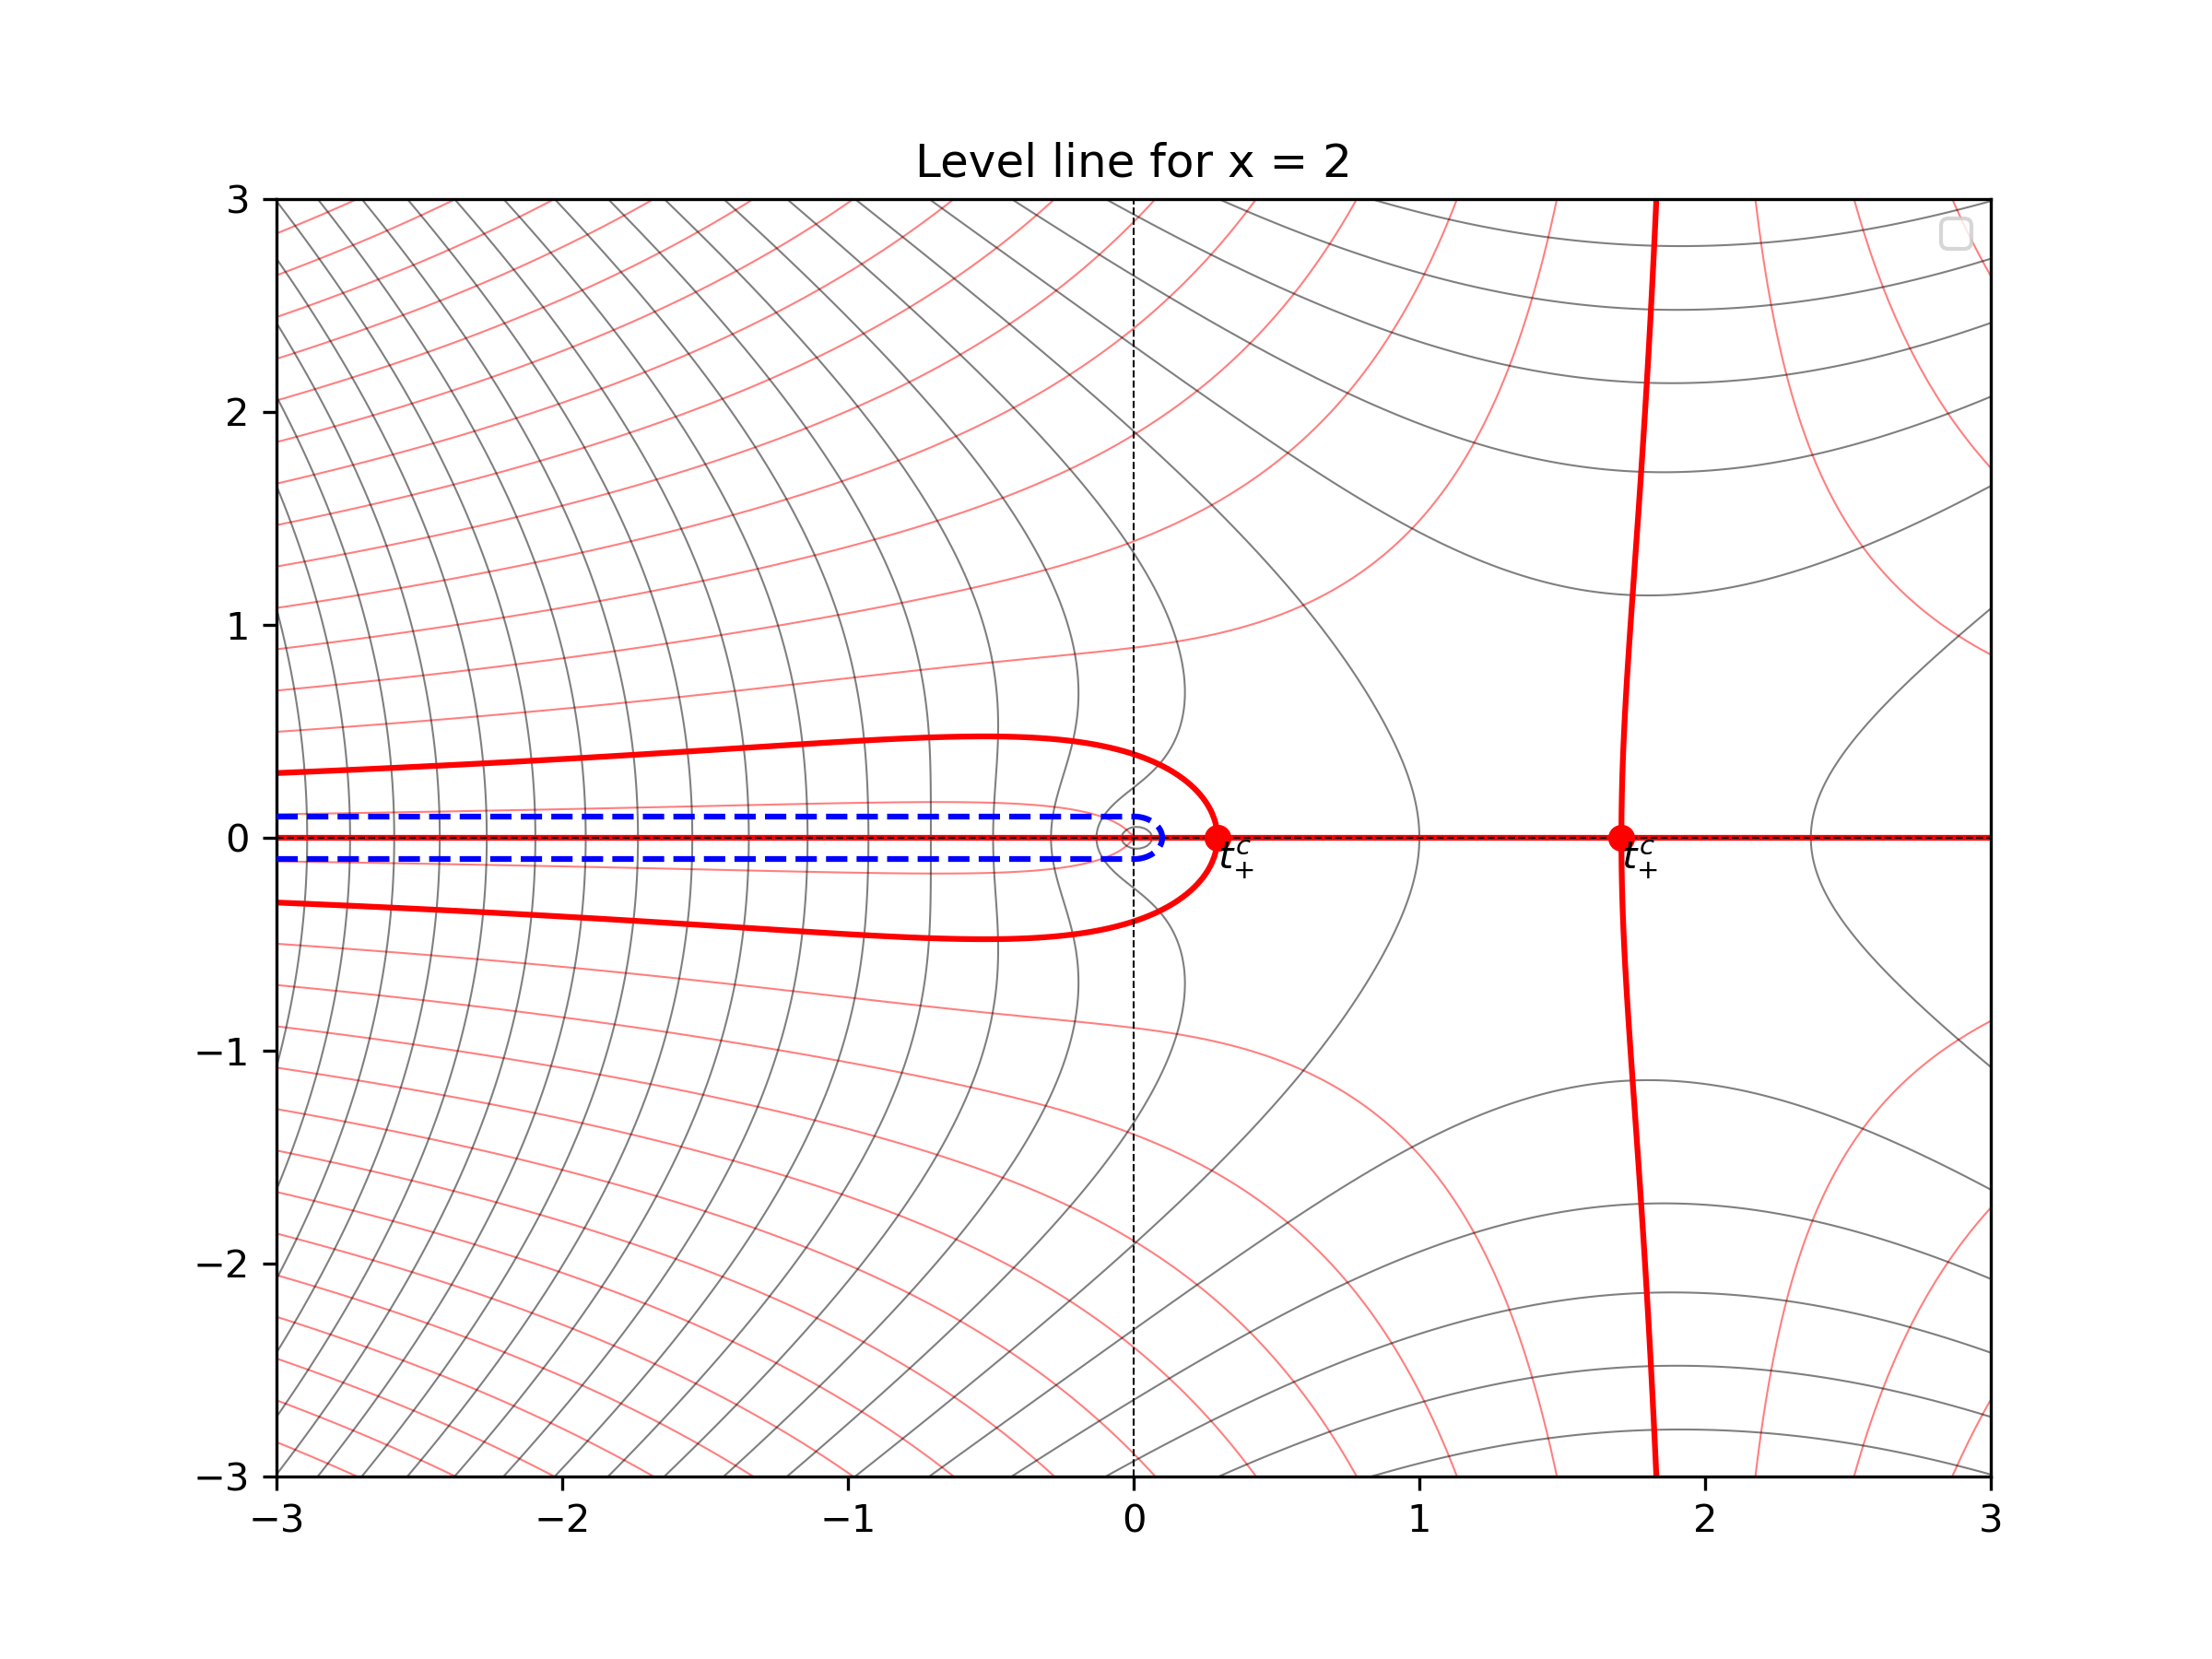
\includegraphics[width=0.49\textwidth]{/home/jvap/Documents/g-contour_plot_theta_2.png}}
	\subfigure{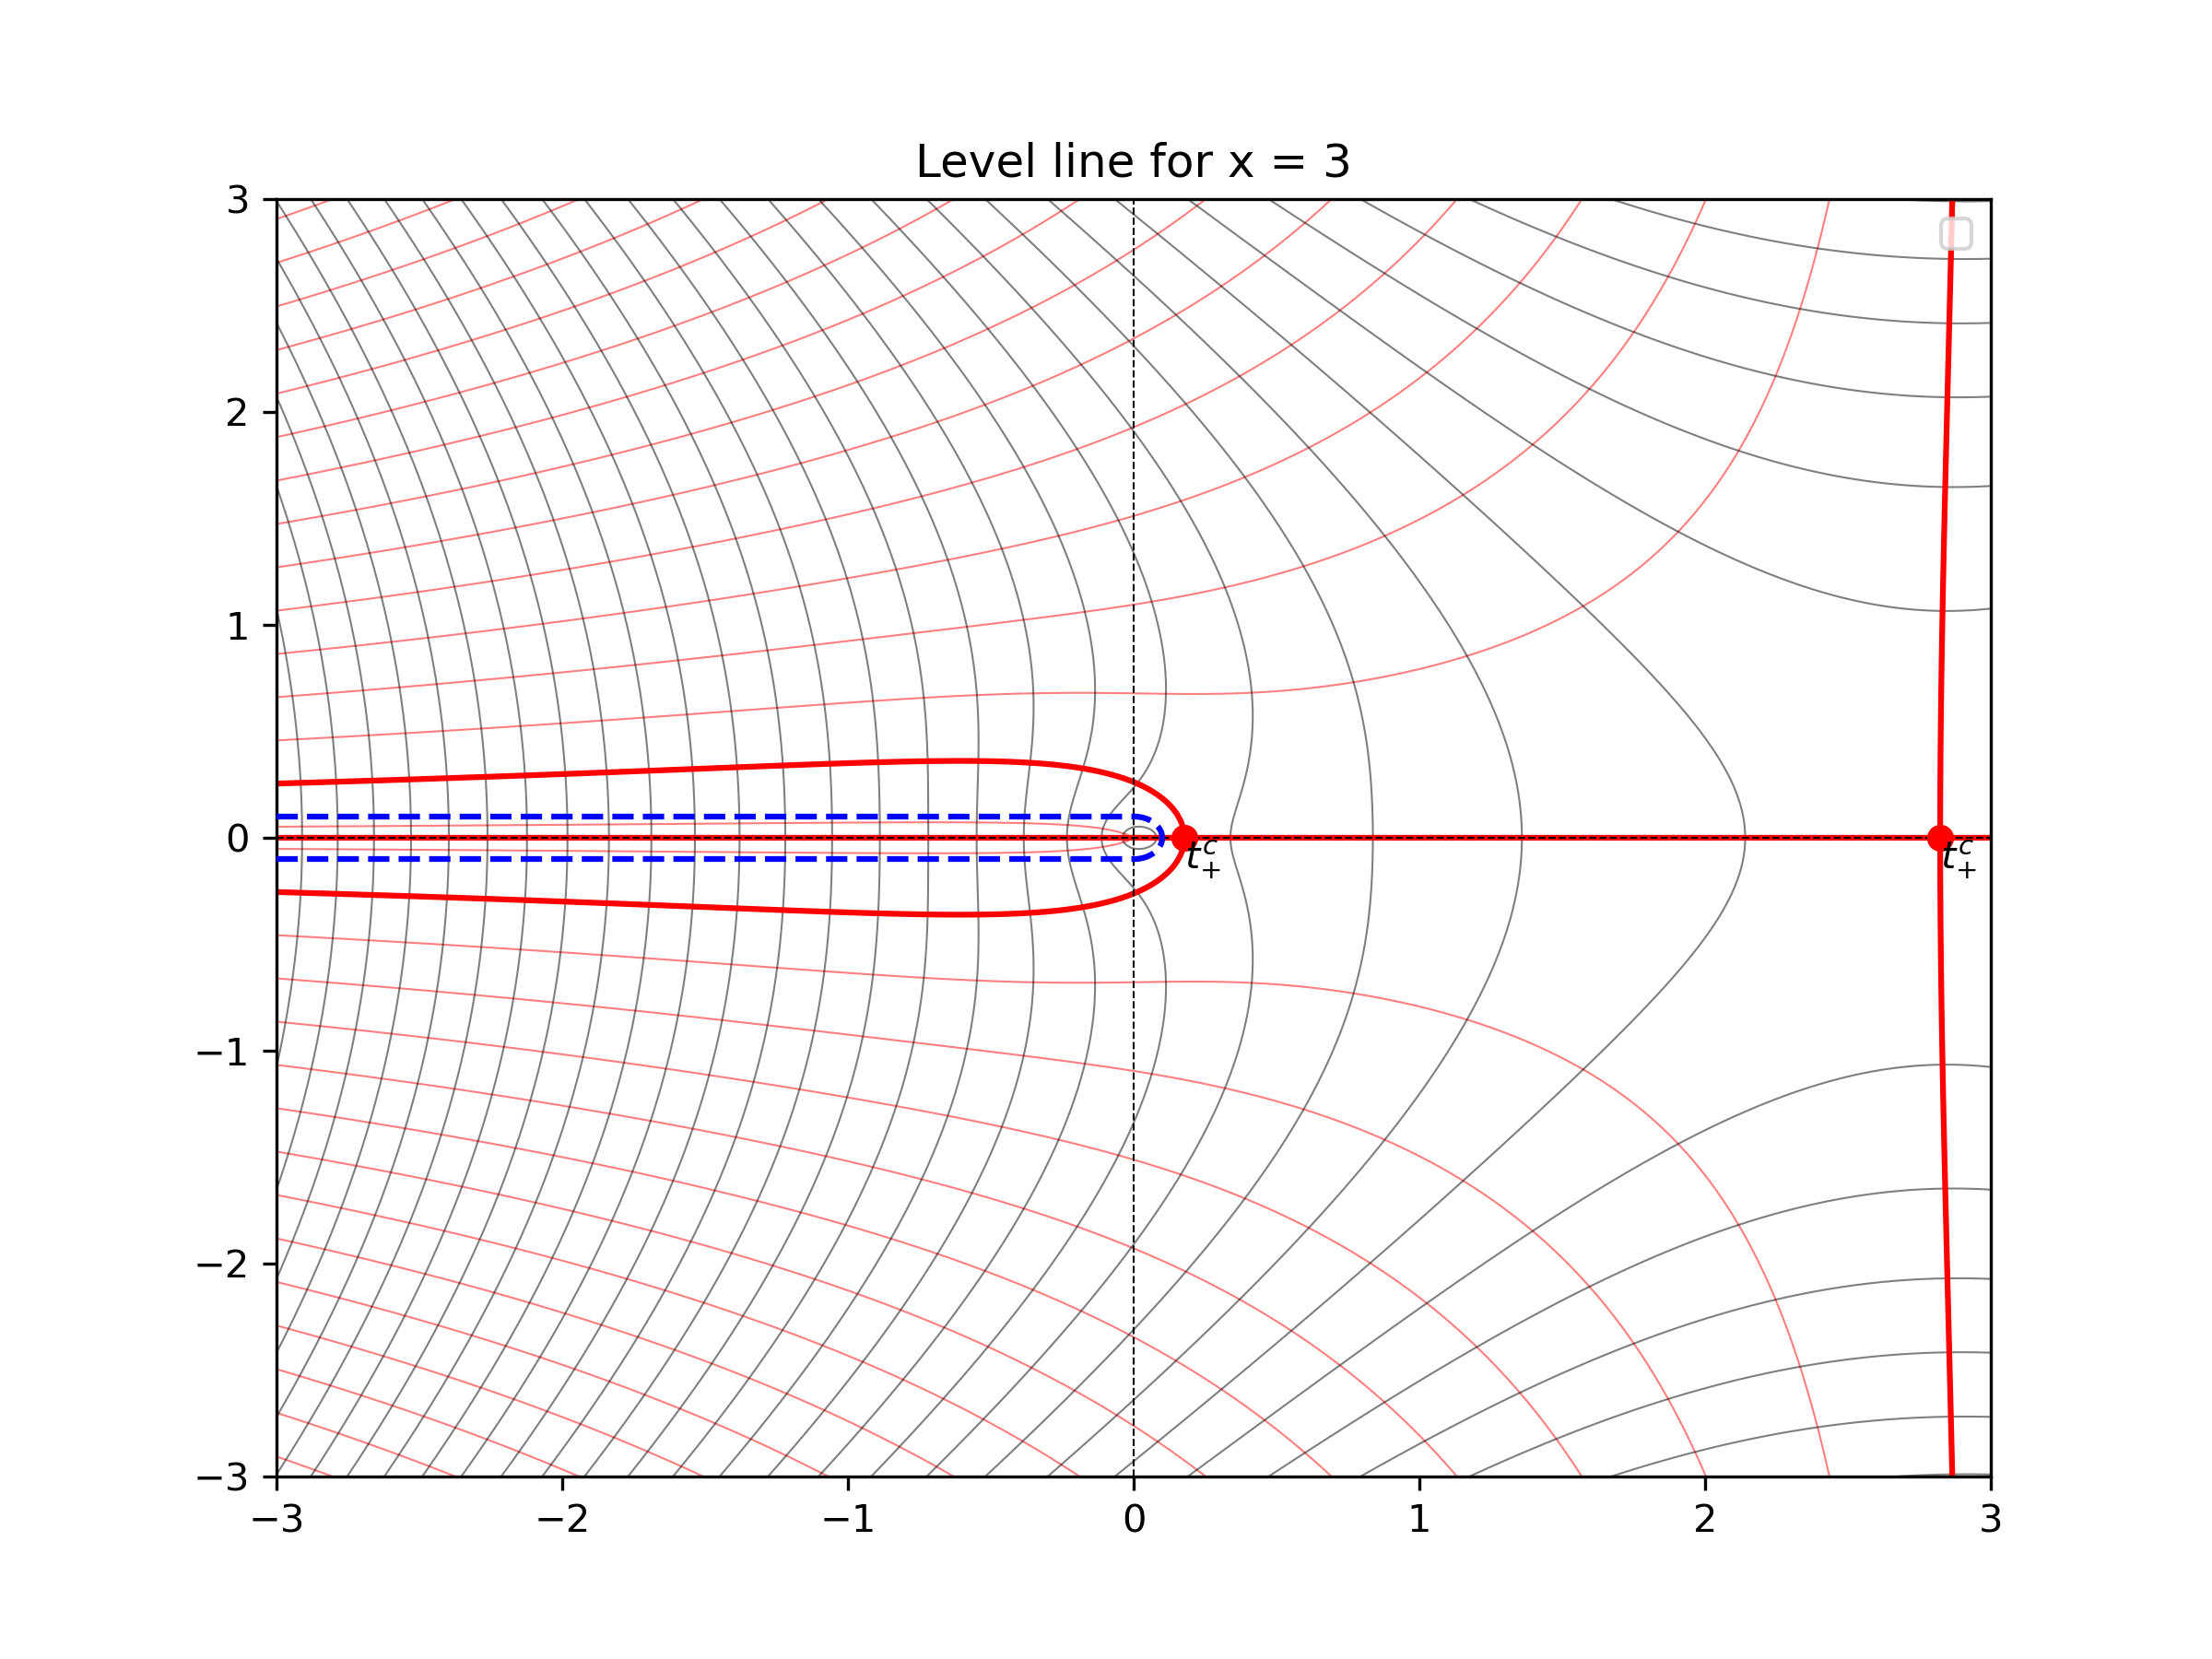
\includegraphics[width=0.49\textwidth]{/home/jvap/Documents/g-contour_plot_theta_3.png}}
	\caption{Scenarios for $x$}
	\label{Fig: x cases for hermite}
\end{figure}

\chapter{Miscellaneous}

\section{Laplace Transform}

\section{Fourrier Transform}

We start by defining what we call a Fourrier Series. Take $f(x)$ to be a a-periodic function, i.e., $f(x+a) = f(x), \ \forall \ x \in \R$. How to characterize such a function? We may try to specify the values it takes on the interval but that's uncountable big. We can also try to approximate it somehow, one such approach is to use geometric periodic functions. We write:
$$
f(x) = \sum_{n=1}^{\infty} \alpha_n \sin\left( \frac{2\pi n x}{a}\right) + \sum_{m=1}^{\infty} \beta_m \cos\left( \frac{2\pi m x}{a}\right) = \sum_{-\infty}^{\infty} f_n \ee^{2 \pi \ii n \frac{x}{a}}
$$

Note that such a summation must be a-periodic as all functions used are a-periodic. Of course, not all functions are guarantee to be expressed in such a way. A know class that works, and usually enough for our purposes, are square-integrable functions, for which
$$
\int_{-a/2}^{a/2} |f(x)|^2 \dd x
$$
exists and is finite. The concept we have is useful but limited if used as such. We want to extend such a concept for functions that are not a-periodic - but how? Define a family of functions $\{f_a(x) | a \in \R^+\}$  such that $f_a(x)$ is a-periodic and $ \lim_{a \rightarrow \infty}f_a(x) = f(x)$. We have that every function $f_{a}$ in the family can be written as a Fourrier Series as it is periodic, so we write:
$$
f_a(x) = \sum_{-\infty}^{\infty} f_{an} \ee^{\ii k_n x}: \ k_n = n \Delta k; \Delta k = \frac{2\pi}{a}.
$$
And as we know about the limit, we can write
\begin{equation}
\begin{split}
	f(x) & = \lim_{a \rightarrow \infty} \left[ \sum_{-\infty}^{\infty} f_{an} \ee^{\ii k_n x} \right] = \lim_{a \rightarrow \infty} \left[ \sum_{-\infty}^{\infty} \frac{\Delta k}{2\pi} \ee^{\ii k_n x} \left( \frac{2\pi f_{an}}{\Delta k}\right) \right] \\
	& = \int_{-\infty}^{\infty} \frac{\dd k}{2\pi} \ee^{\ii k x} F(k); \ \ \text{where} \ \ F(k) = \lim_{a \rightarrow \infty} \left[ \frac{2\pi f_{an}}{\Delta k} \right].
\end{split} 
\end{equation}
where we call $F(x)$ the Fourrier Tranform of the function $f(x)$. We can also define the inverse transform 
\begin{equation}
	\begin{split}
		F(k) & = \lim_{a \rightarrow \infty} \left[ \frac{2\pi}{\Delta k} f_{an}(x) \right] \\
		& = \lim_{a \rightarrow \infty} \left[ \frac{2\pi}{\frac{2\pi}{a}} \frac{1}{a} \int_{-a/2}^{a/2} \dd x \ee^{- \ii k_n x} \right] \\
		& = \int_{-\infty}^{\infty} \dd x \ee^{- \ii k x} f(x)
	\end{split} 
\end{equation}

With this definition we can make explicit some properties of the transform, namely:

\begin{enumerate}
	\item Linearity: Given $f(x)$ and $g(x)$, with its respective $F(x)$ and $G(x)$ Fourrier Tranforms we have that $$a f(x) + b g(x) \rightarrow_{FT} a F(k) + b G(k);$$
	\item Translation: Given $f(x)$ translated by $b$ we write  $$f(x + b) \rightarrow_{FT} \ee^{ikb} F(k);$$
	\item Derivative: Given $f(x)$ we have that the derivative is written $$\frac{\dd}{\dd x}f(x) \rightarrow_{FT}  \ii k F(k)$$
\end{enumerate}

\subsection{On Differential Equations}

Take the damped harmonic oscillator subjected to an additional force $f(t)$. The equation of motion is given by 
$$
\frac{\dd^2 x(t)}{\dd t} + 2\gamma \frac{\dd x(t)}{\dd t} + \omega_0^2 x(t) = \frac{f(t)}{m}.
$$ 
To solve for $x(t)$ we first take the Fourrier Tranform
$$
-\omega^2 X(\omega) - 2\ii \gamma \omega X(\omega) + \omega_0^2 X(\omega) = \frac{F(\omega)}{m}
$$ 
where now we can reorganize to solve for $X(\omega)$.
$$
X(t) = \frac{\frac{F(\omega)}{m}}{-\omega^2 - 2\ii \gamma \omega + \omega_0^2}.
$$
Now it is a simple case of taking the inverse of the Fourrier Transform
$$
x(t) = \int_{-\infty}^{\infty} \frac{\dd \omega}{2\pi} \frac{\frac{\ee^{-i\omega t} F(\omega)}{m}}{-\omega^2 - 2\ii \gamma \omega + \omega_0^2}; \ \ \text{where} \ F(\omega) = \int_{-\infty}^{\infty} \dd t \ee^{\ii \omega t} f(t)  
$$




\end{document}          
